\chapter{Probability and Distribution}
\label{chap:probability}
\markboth{Probability and Distribution}{Probability and Distribution}

\begin{remark}[Positioning of this chapter]\label{rem:probability_chapter_positioning}
This chapter systematically establishes the basic framework of probability theory and distribution theory, focusing on random variables and distribution functions, common distribution families and their interrelations, the unification of characteristic functions with the Fourier transform, Bayesian inference, the basic types of stochastic process, and the laws of large numbers and the central limit theorem.

\textbf{Core interface with periodic mathematics}: probability theory and periodic mathematics meet in depth on four levels. First, \textbf{the characteristic function of a probability distribution is precisely the Fourier transform of the distribution} (Theorem \ref{thm:characteristic_fourier}), and the entire information of a distribution is encoded in the modulus and the phase of its characteristic function, in complete isomorphism with the spectral analysis of periodic functions. Second, \textbf{the uniform distribution on the circle $S^1$ is the Haar measure on the circle group} (Definition \ref{def:uniform_distribution}), and its rotation invariance is precisely the realisation of $U(1)$-symmetry at the probabilistic level. Third, \textbf{probability distributions on the cyclic group $C_N$} (Proposition \ref{prop:discrete_cyclic}) together with periodic sequences, the discrete Fourier transform and circular convolution form a complete algebraic--probabilistic correspondence. Fourth, \textbf{stationary processes and cyclostationary processes} (Definition \ref{def:stationary_process}, \ref{ch14_cyclostationary}) are the action of the time-translation group on stochastic processes, and the spectral decomposition of their autocovariance function (Definition \ref{def:power_spectral_density}) and the power spectrum are the core tools of periodic mathematics at the stochastic level.

\textbf{Guide to the seven themes of this chapter}: translation---the statistical invariance of stationary processes under the action of the time-translation group $\mathbb{Z}$ (discrete) or $\mathbb{R}$ (continuous) (Definition \ref{def:stationary_process}), together with the advance of sequential Bayesian updating along the time axis (Definition \ref{def:sequential_bayesian}); scaling---the scale invariance of self-similar processes and heavy-tailed distributions under the scaling transformation $t\mapsto\lambda t$ (Hurst exponent $H$, tail exponent $\alpha$, Definition \ref{ch14_scale_invariance}), together with the scaling convergence of the central limit theorem (Theorem \ref{thm:central_limit_theorem}); rotation---the phase information of the argument $\arg\phi_X(t)$ of the characteristic function in frequency space (Remark \ref{prop:characteristic_grammar}), and the rotational symmetry of the uniform distribution on $S^1$ (Definition \ref{def:uniform_distribution}); conservation---the invariance of the autocovariance under time translation (Proposition \ref{ch14_autocovariance_stationarity}) and the invariance of the scaling exponent under the scaling transformation; symmetry---the symmetry of distribution families under the prior/likelihood/posterior tripartite structure (the closure of conjugate priors, Definition \ref{def:conjugate_prior}); closure---the convergence closure of the laws of large numbers and the central limit theorem (Theorem \ref{thm:weak_law_of_large_numbers}, \ref{thm:central_limit_theorem}) and the closure criterion `time average $=$ space average' for ergodic orbits (Theorem \ref{thm:birkhoff_ergodic}); period---the period $T$ of a cyclostationary process (Definition \ref{ch14_cyclostationary}) and the periodic pattern of Markov-chain eigenvalues with $|\lambda_i|=1$ (Proposition \ref{prop:transfer_operator_eigen}).
\end{remark}

\begin{figure}[htbp]
\centering
\begin{tikzpicture}[
  font=\small,
  box/.style={draw, rounded corners, fill=blue!8, minimum width=2.6cm, minimum height=0.8cm, align=center},
  sub/.style={draw, rounded corners, fill=green!10, minimum width=2.4cm, minimum height=0.7cm, align=center, font=\footnotesize},
  arr/.style={->, thick, >=stealth}
]
  % First row: the core of probability theory
  \node[box] (prob) {Probability space\\$(\Omega,\mathcal F,\mathbb P)$};
  \node[box, right=0.8cm of prob] (rv) {Random variable\\distribution function};
  \node[box, right=0.8cm of rv] (cf) {Characteristic function\\Fourier transform};
  \node[box, right=0.8cm of cf] (dist) {Common distribution\\families and relations};
  % Second row: the interface with periodic mathematics
  \node[sub, below=1.0cm of prob] (stat) {Stationary process\\time-translation invariant};
  \node[sub, below=1.0cm of rv] (cyc) {Cyclostationary\\period-translation invariant};
  \node[sub, below=1.0cm of cf] (ss) {Self-similar\\scale invariant};
  \node[sub, below=1.0cm of dist] (markov) {Markov chain\\eigenvalue period};
  % Third row: unification
  \node[box, fill=orange!12, below=1.0cm of $(stat)!0.5!(markov)$] (unify) {The unification of probability theory and periodic mathematics: the four main lines of translation/scaling/rotation/period};
  \draw[arr] (prob) -- (rv);
  \draw[arr] (rv) -- (cf);
  \draw[arr] (cf) -- (dist);
  \draw[arr] (prob) -- (stat);
  \draw[arr] (rv) -- (cyc);
  \draw[arr] (cf) -- (ss);
  \draw[arr] (dist) -- (markov);
  \draw[arr] (stat) -- (unify);
  \draw[arr] (cyc) -- (unify);
  \draw[arr] (ss) -- (unify);
  \draw[arr] (markov) -- (unify);
\end{tikzpicture}
\caption{Overview of the structure of this chapter: the core of probability theory (probability space, random variable, characteristic function, distribution families) and the interface with periodic mathematics (stationary, cyclostationary, self-similar, Markov chain), finally unified along four main lines.}
\label{fig:probability_overview}
\end{figure}

\section{Events and Their Probabilities}\label{sec:events_probability}

\subsection{Random Events and Probability}

\begin{definition}[Random event]\label{def:random_event}
In a probability space $(\Omega, \mathcal{F}, \mathbb{P})$, the elements of $\mathcal{F}$ are called \textbf{random events}. The \textbf{probability} $\mathbb{P}(A)$ of an event $A$ is a real number in $[0,1]$ satisfying:
\begin{enumerate}[label=(\roman*)]
    \item \textbf{Non-negativity}: $\mathbb{P}(A) \ge 0$ holds for all $A \in \mathcal{F}$.
    \item \textbf{Normalisation}: $\mathbb{P}(\Omega) = 1$.
    \item \textbf{Countable additivity}: for a sequence of pairwise disjoint events $\{A_n\}_{n=1}^{\infty}$, we have $\mathbb{P}(\bigcup_{n=1}^{\infty} A_n) = \sum_{n=1}^{\infty} \mathbb{P}(A_n)$.
\end{enumerate}
\end{definition}

\begin{proposition}[Basic properties of the probability measure]\label{prop:probability_measure_properties}
Let $(\Omega, \mathcal{F}, \mathbb{P})$ be a probability space and $A, B \in \mathcal{F}$. Then
\begin{enumerate}[label=(\roman*)]
    \item $\mathbb{P}(\emptyset) = 0$;
    \item \textbf{Monotonicity}: if $A \subseteq B$, then $\mathbb{P}(A) \le \mathbb{P}(B)$;
    \item \textbf{Complementarity}: $\mathbb{P}(A^c) = 1 - \mathbb{P}(A)$;
    \item \textbf{Finite additivity}: if $A \cap B = \emptyset$, then $\mathbb{P}(A \cup B) = \mathbb{P}(A) + \mathbb{P}(B)$.
\end{enumerate}
\end{proposition}

\begin{proof}
(i) Take $A_n = \emptyset$ ($n \ge 1$); by countable additivity $\mathbb{P}(\emptyset) = \sum_{n=1}^{\infty}\mathbb{P}(\emptyset)$, hence $\mathbb{P}(\emptyset) = 0$.
(ii) If $A \subseteq B$, then $B = A \cup (B \setminus A)$ is a disjoint union, so $\mathbb{P}(B) = \mathbb{P}(A) + \mathbb{P}(B \setminus A) \ge \mathbb{P}(A)$.
(iii) $\Omega = A \cup A^c$ is disjoint, so by normalisation $1 = \mathbb{P}(\Omega) = \mathbb{P}(A) + \mathbb{P}(A^c)$.
(iv) Let $A_1 = A$, $A_2 = B$ and $A_n = \emptyset$ ($n \ge 3$); countable additivity together with (i) gives $\mathbb{P}(A \cup B) = \mathbb{P}(A) + \mathbb{P}(B)$.
\end{proof}

\begin{figure}[htbp]
\centering
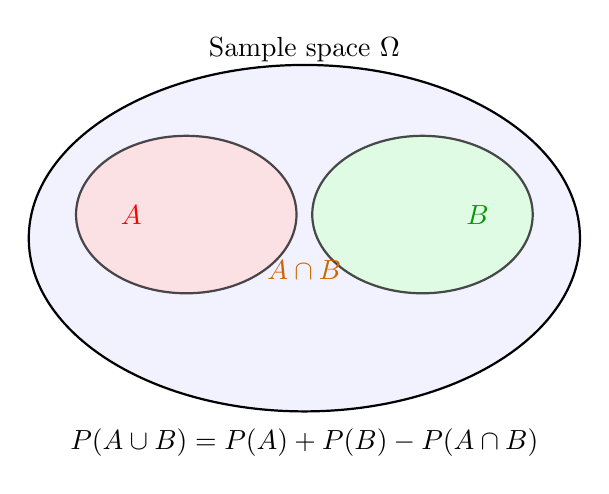
\begin{tikzpicture}[scale=1.0]
  % Sample space
  \draw[thick, fill=blue!5] (0,0) ellipse (3.5 and 2.2);
  \node at (0,2.4) {Sample space $\Omega$};
  % Event A
  \draw[thick, fill=red!15, opacity=0.7] (-1.5,0.3) ellipse (1.4 and 1.0);
  \node[red] at (-2.2,0.3) {$A$};
  % Event B
  \draw[thick, fill=green!15, opacity=0.7] (1.5,0.3) ellipse (1.4 and 1.0);
  \node[green!60!black] at (2.2,0.3) {$B$};
  % Intersection
  \begin{scope}
    \clip (-1.5,0.3) ellipse (1.4 and 1.0);
    \fill[orange!40, opacity=0.7] (1.5,0.3) ellipse (1.4 and 1.0);
  \end{scope}
  \node[orange!80!black] at (0,-0.4) {$A\cap B$};
  % Explanation
  \node at (0,-2.6) {$\mathbb P(A\cup B)=\mathbb P(A)+\mathbb P(B)-\mathbb P(A\cap B)$};
\end{tikzpicture}
\caption{Venn diagram of events and the addition formula: $\mathbb{P}(A\cup B)=\mathbb{P}(A)+\mathbb{P}(B)-\mathbb{P}(A\cap B)$.}
\label{fig:venn_diagram}
\end{figure}

\begin{definition}[The relation between frequency and probability]\label{def:frequency_probability}
Let the event $A$ occur $n_A$ times in $n$ independent repeated trials. The \textbf{frequency} of $A$ is defined as $f_n(A) = n_A / n$. By the law of large numbers, the frequency converges in probability to the probability: $\lim_{n \to \infty} f_n(A) = \mathbb{P}(A)$. The frequency is the empirical estimate of the probability, and the probability is the limit of the frequency.
\end{definition}

\subsection{Formulae for Calculating Probabilities}

\begin{definition}[Addition formula]\label{def:addition_rule}
For any two events $A$ and $B$, $\mathbb{P}(A \cup B) = \mathbb{P}(A) + \mathbb{P}(B) - \mathbb{P}(A \cap B)$.
\end{definition}

\begin{definition}[Conditional probability and the multiplication formula]\label{def:conditional_multiplication}
If $\mathbb{P}(B) > 0$, then
\[
\mathbb{P}(A \mid B) = \frac{\mathbb{P}(A \cap B)}{\mathbb{P}(B)}, \quad \mathbb{P}(A \cap B) = \mathbb{P}(A \mid B) \mathbb{P}(B).
\]
\end{definition}

\begin{definition}[The law of total probability and Bayes' formula]\label{def:total_probability_bayes}
Let $\{B_i\}_{i=1}^n$ be a partition of the sample space $\Omega$ with $\mathbb{P}(B_i) > 0$. Then
\[
\mathbb{P}(A) = \sum_{i=1}^n \mathbb{P}(A \mid B_i) \mathbb{P}(B_i),
\]
\[
\mathbb{P}(B_i \mid A) = \frac{\mathbb{P}(A \mid B_i) \mathbb{P}(B_i)}{\sum_{j=1}^n \mathbb{P}(A \mid B_j) \mathbb{P}(B_j)}.
\]
\end{definition}

\begin{definition}[Independence of events]\label{def:independence}
Events $A$ and $B$ are called \textbf{independent} if $\mathbb{P}(A \cap B) = \mathbb{P}(A)\mathbb{P}(B)$. Independence means that the occurrence of one event does not change the conditional probability of the other.
\end{definition}

\section{Random Variables and Distribution Functions}\label{sec:random_variables}

\subsection{Random Variables}

\begin{definition}[Random variable]\label{def:random_variable}
Let $(\Omega, \mathcal{F}, \mathbb{P})$ be a probability space and $(\mathcal{X}, \mathcal{B})$ a measurable space. A \textbf{random variable} is a measurable mapping $X: \Omega \to \mathcal{X}$, that is, $X^{-1}(B) \in \mathcal{F}$ for every $B \in \mathcal{B}$.

When $\mathcal{X} = \mathbb{R}$ and $\mathcal{B} = \mathcal{B}(\mathbb{R})$, $X$ is called a real-valued random variable; when $\mathcal{X} = \mathbb{Z}/N\mathbb{Z}$ or $\mathcal{X}$ is finite, $X$ is called a discrete random variable.
\end{definition}

\begin{remark}[On the use of the terms `phase space' and `phase encoding']\label{rem:phase_terminology_usage}
In the probabilistic framework of this section, the sample space $\Omega$ is sometimes understood as the `phase space' of a periodic system, and a random variable is sometimes understood as a `phase encoding'. Elsewhere in this book these terms are completely equivalent to `sample space' and `random variable'; they serve only to keep the terminology consistent with that of the other chapters. In this chapter and in the subsequent discussion the two may be used interchangeably, and they do not constitute a new mathematical concept. For instance, for values taken in the finite cyclic group $C_N = \mathbb{Z}/N\mathbb{Z} = \{0, 1, \dots, N-1\}$, the group $C_N$ is the sample space and $k \mapsto \mathbb{P}(X = k)$ is the probability mass function.
\end{remark}

\begin{example}[A basic example of a finite sample space]\label{ex:finite_sample_space}
$C_2 = \{0, 1\}$ is the smallest non-trivial finite sample space. The Bernoulli distribution $\mathbb{P}(X=1) = p$, $\mathbb{P}(X=0) = 1-p$ is a probability distribution on $C_2$. A distribution $(p_0, p_1, \dots, p_9)$ on $C_{10} = \{0, 1, \dots, 9\}$ gives a probability on the decimal digits.
\end{example}

\subsection{Cumulative Distribution Functions}

\begin{definition}[Cumulative distribution function]\label{def:cdf}
Let $X$ be a real-valued random variable. The \textbf{cumulative distribution function} (CDF) of $X$ is defined as
\[
F_X(x) = \mathbb{P}(X \le x), \qquad x \in \mathbb{R}.
\]
\end{definition}

\begin{property}[Basic properties of the cumulative distribution function]\label{prop:cdf_properties}
Let $F_X$ be the cumulative distribution function of a random variable $X$. Then
\begin{enumerate}[label=(\roman*)]
    \item \textbf{Monotonically non-decreasing}: if $x_1 \le x_2$, then $F_X(x_1) \le F_X(x_2)$.
    \item \textbf{Right-continuous}: $\lim_{h \to 0^+} F_X(x+h) = F_X(x)$.
    \item \textbf{Limiting behaviour}: $\lim_{x \to -\infty} F_X(x) = 0$, $\lim_{x \to +\infty} F_X(x) = 1$.
    \item \textbf{Interval probability}: $\mathbb{P}(a < X \le b) = F_X(b) - F_X(a)$.
\end{enumerate}
\end{property}

\begin{proof}
(i) By monotonicity (Proposition \ref{prop:probability_measure_properties} (ii)), the event $\{X \le x_1\} \subseteq \{X \le x_2\}$, hence $F_X(x_1) \le F_X(x_2)$.

(ii) Let $x_n \downarrow x$; then the sequence of events $\{X \le x_n\}$ is decreasing with intersection $\{X \le x\}$, so by the continuity of probability $F_X(x_n) \to F_X(x)$.

(iii) As $x \to -\infty$ the sequence of events $\{X \le x\}$ decreases to the empty set, so $F_X \to 0$; as $x \to +\infty$ it increases to $\Omega$, so $F_X \to 1$.

(iv) $\{X \le b\} = \{X \le a\} \cup \{a < X \le b\}$ is a disjoint union, hence $F_X(b) = F_X(a) + \mathbb{P}(a < X \le b)$.
\end{proof}

\begin{figure}[htbp]
\centering
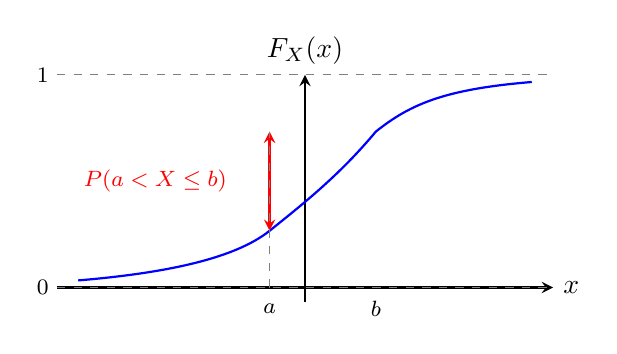
\begin{tikzpicture}[scale=0.9]

  \draw[->, thick, >=stealth] (-3.5,0) -- (3.5,0) node[right] {$x$};
  \draw[->, thick, >=stealth] (0,-0.2) -- (0,3) node[above] {$F_X(x)$};

  \draw[thick, blue] (-3.2,0.1) .. controls (-2,0.2) and (-1,0.4) .. (-0.5,0.8)
                                .. controls (0,1.2) and (0.5,1.6) .. (1,2.2)
                                .. controls (1.5,2.6) and (2,2.8) .. (3.2,2.9);

  \draw[gray, dashed] (-3.5,0) -- (3.5,0);
  \draw[gray, dashed] (-3.5,3) -- (3.5,3);
  \node[font=\footnotesize] at (-3.7,0) {$0$};
  \node[font=\footnotesize] at (-3.7,3) {$1$};

  \draw[<->, thick, red, >=stealth] (-0.5,0.8) -- (-0.5,2.2);
  \node[red, font=\footnotesize, xshift=-1cm] at (-1.0,1.5) {$\mathbb P(a<X\le b)$};
  \draw[gray, dashed] (-0.5,0) -- (-0.5,2.2);
  \node[font=\footnotesize] at (-0.5,-0.3) {$a$};
  \node[font=\footnotesize] at (1,-0.3) {$b$};
\end{tikzpicture}
\caption{Properties of the cumulative distribution function: monotonically non-decreasing, right-continuous, with interval probabilities given by the difference of the endpoints.}
\label{fig:cdf_properties}
\end{figure}

\begin{theorem}[The one-to-one correspondence between CDFs and distributions]\label{thm:cdf_uniqueness}
Two random variables $X$ and $Y$ have the same distribution if and only if their cumulative distribution functions are equal: $F_X = F_Y$.
\end{theorem}

\begin{proof}
Necessity: if $X\stackrel{d}{=}Y$, then $\mathbb P(X\le x)=\mathbb P(Y\le x)$ for all $x$, that is, $F_X=F_Y$. Sufficiency: suppose $F_X = F_Y$. For any $a < b$, Property \ref{prop:cdf_properties}(iv) gives $\mathbb{P}(a < X \le b) = \mathbb{P}(a < Y \le b)$. For any half-open interval $(a, b]$ the two random variables have equal probability. The $\sigma$-algebra generated by the family of half-open intervals is the Borel $\sigma$-algebra $\mathcal{B}(\mathbb{R})$, so the two random variables induce the same probability measure on $\mathcal{B}(\mathbb{R})$, that is, they are identically distributed.
\end{proof}

\begin{definition}[Quantile function]\label{def:quantile}
Let $F_X$ be the cumulative distribution function of a random variable $X$. The \textbf{quantile function} (generalised inverse) of $X$ is defined as
\[
F_X^{-1}(p) = \inf\{x \in \mathbb{R} : F_X(x) \ge p\}, \qquad p \in (0, 1).
\]
In particular, $F_X^{-1}(1/2)$ is called the \textbf{median}, whilst $F_X^{-1}(1/4)$ and $F_X^{-1}(3/4)$ are called the first and the third quartile respectively.
\end{definition}

\begin{proposition}[Basic properties of the quantile function]\label{prop:quantile_properties}
Let $F_X^{-1}$ be the quantile function of a random variable $X$. Then
\begin{enumerate}[label=(\roman*)]
    \item \textbf{Monotonically non-decreasing}: $p_1 \le p_2 \Rightarrow F_X^{-1}(p_1) \le F_X^{-1}(p_2)$.
    \item \textbf{Left-continuous}: $F_X^{-1}$ is left-continuous on $(0,1)$.
    \item \textbf{Adjoint relation with the CDF}: $F_X^{-1}(p) \le x \iff p \le F_X(x)$.
\end{enumerate}
\end{proposition}

\begin{proof}
(i) If $p_1 \le p_2$, then $\{x : F_X(x) \ge p_2\} \subseteq \{x : F_X(x) \ge p_1\}$, so the infimum is monotone.

(ii) Let $p_n \uparrow p$. By (i), $F_X^{-1}(p_n)$ is increasing and $\le F_X^{-1}(p)$. Let its limit be $L \le F_X^{-1}(p)$. By the equivalence to be proved in (iii), $F_X^{-1}(p_n) \le x \iff p_n \le F_X(x)$. Taking $x = L$, right-continuity gives $p \le F_X(L)$, hence $F_X^{-1}(p) \le L$, and therefore $L = F_X^{-1}(p)$.

(iii) If $p \le F_X(x)$, then $x \in \{y : F_X(y) \ge p\}$, so $F_X^{-1}(p) \le x$. Conversely, if $F_X^{-1}(p) \le x$, then from the monotone non-decrease of $F_X$ and $F_X(F_X^{-1}(p)) \ge p$ we obtain $F_X(x) \ge p$.
\end{proof}

\subsection{Discrete and Continuous Distributions}

\begin{definition}[Discrete distribution]\label{def:discrete_distribution}
Let $X$ be a random variable taking values in a finite or countable set $\{x_0 < x_1 < \cdots\}$. The \textbf{probability mass function} (PMF) of $X$ is $p_X(k) = \mathbb{P}(X = x_k)$, satisfying
\[
p_X(k) \ge 0, \quad \sum_{k} p_X(k) = 1.
\]
\end{definition}

\begin{proposition}[The probability mass function and the CDF of a discrete distribution]\label{prop:pmf_cdf_relation}
Let $X$ be a discrete random variable taking values in $\{x_0 < x_1 < \cdots\}$ and let $p_k = \mathbb{P}(X = x_k)$. Then
\[
F_X(x) = \sum_{k : x_k \le x} p_k.
\]
\end{proposition}

\begin{proof}
$\{X \le x\} = \bigcup_{k: x_k \le x} \{X = x_k\}$ is a countable disjoint union, and the result follows from countable additivity.
\end{proof}

\begin{proposition}[Any finite discrete distribution is a distribution on a cyclic group]
\label{prop:discrete_cyclic}
Let $X$ be a discrete random variable taking values in the finite set
\[
\{x_0, x_1, \dots, x_{N-1}\}.
\]
Through the bijection $x_k \mapsto k \in C_N$,
$X$ is equivalent to a probability distribution $(p_0, p_1, \dots, p_{N-1})$ on $C_N$,
where $p_k = \mathbb{P}(X = x_k)$.
\end{proposition}
\begin{proof}
Construct the bijection $\varphi(x_k) = k$. Define $p(k) = \mathbb{P}(X = x_k)$. The total mass is $\sum_{k=0}^{N-1} p(k) = 1$. This is a standard reparametrisation of a probability distribution on a finite set and does not constitute new mathematical content.
\end{proof}

\begin{proposition}[Translation-invariant distribution on the cyclic group]\label{prop:cyclic_uniform}
The only translation-invariant probability distribution on $C_N$ is the uniform distribution $p(k) = 1/N$. For any $a \in C_N$, the condition $p(k+a) = p(k)$ forces $p$ to be constant.
\end{proposition}

\begin{proof}
Translation invariance requires $p(k+a) = p(k)$ for all $k, a \in C_N$. Taking $a=1$ gives $p(k+1) = p(k)$ for all $k$, so $p$ is a constant function. Normalisation gives $p(k) = 1/N$. This is the Haar measure on $C_N$.
\end{proof}

\begin{definition}[Continuous distribution]\label{def:continuous_distribution}
A random variable $X$ is called \textbf{continuous} if there exists a \textbf{probability density function} (PDF) $f_X(x)$ such that $\mathbb{P}(X \in B) = \int_B f_X(x) dx$ holds for all $B \in \mathcal{B}(\mathbb{R})$. The relation between the density and the cumulative distribution function is $F_X(x) = \int_{-\infty}^{x} f_X(t) dt$, and $F_X' = f_X$ wherever $f_X$ is continuous.
\end{definition}

\section{Random Variables and Common Distributions}\label{sec:common_distributions}

\subsection{Discrete Random Variables}

\begin{definition}[The Bernoulli and binomial distributions]\label{def:bernoulli_binomial}
The Bernoulli random variable $X \sim \operatorname{Bernoulli}(p)$ is the distribution on $C_2$ given by $\mathbb{P}(X=1) = p$ and $\mathbb{P}(X=0) = 1-p$.

The number of successes $X \sim \operatorname{Binomial}(n, p)$ in $n$ independent Bernoulli trials is the distribution on $C_{n+1} = \{0, 1, \dots, n\}$:
\[
\mathbb{P}(X = k) = \binom{n}{k} p^k (1-p)^{n-k}, \quad k = 0, 1, \dots, n.
\]
The expectation is $\mathbb{E}[X] = np$ and the variance is $\operatorname{Var}(X) = np(1-p)$.
\end{definition}

\begin{definition}[The Poisson distribution]\label{def:poisson_distribution}
The Poisson distribution $X \sim \operatorname{Poisson}(\lambda)$ is the distribution on $\mathbb{N}$:
\[
\mathbb{P}(X = k) = \frac{\lambda^k e^{-\lambda}}{k!}, \quad k = 0, 1, 2, \dots.
\]
Both the expectation and the variance are $\lambda$. The Poisson distribution is the limiting distribution of the binomial distribution as $n \to \infty$ and $np \to \lambda$.
\end{definition}

\begin{definition}[The geometric and negative binomial distributions]\label{def:geometric_negbinomial}
The geometric distribution $X \sim \operatorname{Geometric}(p)$ is the number of trials required for the first success:
\[
\mathbb{P}(X = k) = (1-p)^{k-1} p, \quad k = 1, 2, \dots.
\]
The expectation is $\mathbb{E}[X] = 1/p$ and the variance is $\operatorname{Var}(X) = (1-p)/p^2$. The geometric distribution has the memoryless property.

The negative binomial distribution $X \sim \operatorname{NegBinomial}(r, p)$ is the number of trials required for the $r$-th success:
\[
\mathbb{P}(X = k) = \binom{k-1}{r-1} p^r (1-p)^{k-r}, \quad k = r, r+1, \dots.
\]
The expectation is $\mathbb{E}[X] = r/p$ and the variance is $\operatorname{Var}(X) = r(1-p)/p^2$.
\end{definition}

\begin{figure}[htbp]
\centering
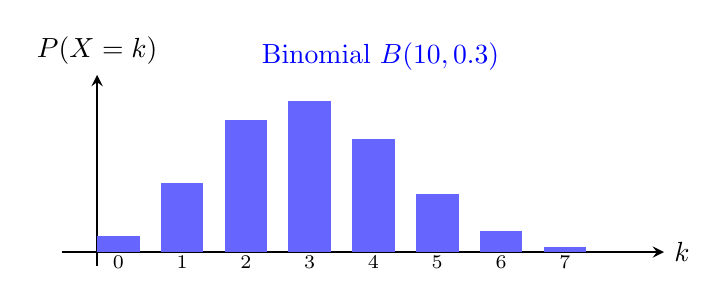
\begin{tikzpicture}[scale=0.9]

  \draw[->, thick, >=stealth] (-0.5,0) -- (8,0) node[right] {$k$};
  \draw[->, thick, >=stealth] (0,-0.2) -- (0,2.5) node[above] {$\mathbb P(X=k)$};

  \foreach \k/\h in {0/0.028,1/0.121,2/0.233,3/0.267,4/0.200,5/0.103,6/0.037,7/0.009} {
    \fill[blue!60] (\k*0.9,0) rectangle (\k*0.9+0.6,\h*8);
    \node[font=\scriptsize] at (\k*0.9+0.3,-0.15) {\k};
  }
  \node[blue, yshift=0.5cm] at (4,2.2) {Binomial $B(10,0.3)$};
\end{tikzpicture}
\caption{The probability mass function of the binomial distribution $B(10,0.3)$.}
\label{fig:binomial_pmf}
\end{figure}

\subsection{Continuous Random Variables}

\begin{definition}[The uniform distribution]\label{def:uniform_distribution}
The density of $X \sim \operatorname{Uniform}(a, b)$ is $f_X(x) = \frac{1}{b-a}$ ($a \le x \le b$). The uniform distribution on $S^1$ is the Haar measure on the circle group and possesses full rotational symmetry.
\end{definition}

\begin{proposition}[Rotation invariance of the uniform distribution on $S^1$]\label{prop:S1_uniform_rotation}
Let $X$ be uniformly distributed on $S^1 = \mathbb{R}/(2\pi\mathbb{Z})$ (density $f_X(\theta) = 1/(2\pi)$). Then for any $\phi \in S^1$, the variable $X + \phi$ (modulo $2\pi$) is still uniformly distributed. The uniform distribution on $S^1$ is the only probability distribution with rotation invariance.
\end{proposition}

\begin{proof}
The density is $f_{X+\phi}(\theta) = f_X(\theta - \phi) = 1/(2\pi)$, which is independent of $\phi$. Conversely, if $f$ is rotation invariant, then $f(\theta - \phi) = f(\theta)$ for all $\phi$, so $f$ is constant, and normalisation gives $f = 1/(2\pi)$.
\end{proof}

\begin{definition}[The normal distribution]\label{def:normal_distribution}
The density of $X \sim \mathcal{N}(\mu, \sigma^2)$ is
\[
f_X(x) = \frac{1}{\sqrt{2\pi}\sigma} e^{-(x-\mu)^2/(2\sigma^2)}.
\]
Here $\mu$ is the expectation and $\sigma^2$ is the variance. The normal distribution is the limiting distribution of the central limit theorem.
\end{definition}

\begin{definition}[The exponential distribution]\label{def:exponential_distribution}
The density of $X \sim \operatorname{Exponential}(\lambda)$ is $f_X(x) = \lambda e^{-\lambda x}$ ($x \ge 0$). It has the memoryless property: $\mathbb{P}(X > s + t \mid X > s) = \mathbb{P}(X > t)$. The expectation is $1/\lambda$ and the variance is $1/\lambda^2$.
\end{definition}

\begin{definition}[The gamma distribution]\label{def:gamma_distribution}
The density of $X \sim \operatorname{Gamma}(\alpha, \beta)$ is
\[
f_X(x) = \frac{\beta^\alpha}{\Gamma(\alpha)} x^{\alpha-1} e^{-\beta x}, \quad x > 0,
\]
where $\alpha > 0$ is the shape parameter and $\beta > 0$ is the rate parameter, and $\Gamma(\alpha) = \int_0^\infty t^{\alpha-1} e^{-t} dt$ is the gamma function. The expectation is $\alpha/\beta$ and the variance is $\alpha/\beta^2$. The exponential distribution is the special case $\alpha = 1$.
\end{definition}

\begin{definition}[The beta distribution]\label{def:beta_distribution}
The density of $X \sim \operatorname{Beta}(\alpha, \beta)$ is
\[
f_X(x) = \frac{x^{\alpha-1} (1-x)^{\beta-1}}{B(\alpha, \beta)}, \quad x \in (0, 1),
\]
where $B(\alpha, \beta) = \Gamma(\alpha)\Gamma(\beta)/\Gamma(\alpha+\beta)$ is the beta function. The expectation is $\alpha/(\alpha+\beta)$ and the variance is $\alpha\beta/[(\alpha+\beta)^2(\alpha+\beta+1)]$. The uniform distribution $\operatorname{Uniform}(0,1)$ is the special case $\alpha = \beta = 1$.
\end{definition}

\begin{definition}[The chi-squared, $t$, and $F$ distributions]\label{def:chi2_t_f}
Let $Z_1, \dots, Z_n$ be independent standard normal random variables.
\begin{enumerate}[label=(\roman*)]
    \item \textbf{Chi-squared distribution}: $X = \sum_{i=1}^n Z_i^2 \sim \chi^2(n)$, the special case $\operatorname{Gamma}(n/2, 1/2)$, with expectation $n$ and variance $2n$.
    \item \textbf{$t$ distribution}: if $Z \sim \mathcal{N}(0,1)$ and $V \sim \chi^2(n)$ are independent, then $T = Z/\sqrt{V/n} \sim t(n)$, with expectation $0$ ($n > 1$) and variance $n/(n-2)$ ($n > 2$).
    \item \textbf{$F$ distribution}: if $U \sim \chi^2(m)$ and $V \sim \chi^2(n)$ are independent, then $F = (U/m)/(V/n) \sim F(m, n)$.
\end{enumerate}
\end{definition}

\begin{figure}[htbp]
\centering
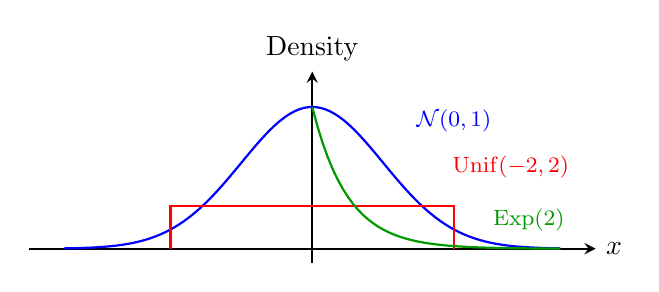
\begin{tikzpicture}[scale=0.9]

  \draw[->, thick, >=stealth] (-4,0) -- (4,0) node[right] {$x$};
  \draw[->, thick, >=stealth] (0,-0.2) -- (0,2.5) node[above] {Density};

  \draw[thick, blue, domain=-3.5:3.5, samples=100] plot (\x, {2*exp(-\x*\x/2)});
  \node[blue, font=\footnotesize] at (2.0,1.8) {$\mathcal N(0,1)$};

  \draw[thick, red] (-2,0) -- (-2,0.6) -- (2,0.6) -- (2,0);
  \node[red, font=\footnotesize, yshift=0.5cm] at (2.8,0.6) {$\mathrm{Unif}(-2,2)$};

  \draw[thick, green!60!black, domain=0:3.5, samples=50] plot (\x, {2*exp(-2*\x)});
  \node[green!60!black, font=\footnotesize, xshift=0.5cm] at (2.5,0.4) {$\mathrm{Exp}(2)$};
\end{tikzpicture}
\caption{Comparison of the density functions of three continuous distributions: normal, uniform and exponential.}
\label{fig:continuous_pdf}
\end{figure}

\subsection{Relations among Common Distributions}

\begin{proposition}[Limits and special cases of common distributions]\label{prop:distribution_relations}
\begin{enumerate}[label=(\roman*)]
    \item \textbf{Binomial to Poisson}: $\operatorname{Binomial}(n, \lambda/n) \xrightarrow{d} \operatorname{Poisson}(\lambda)$ ($n \to \infty$).
    \item \textbf{Binomial to normal}: $\frac{X - np}{\sqrt{np(1-p)}} \xrightarrow{d} \mathcal{N}(0,1)$ ($n \to \infty$, the De Moivre--Laplace theorem).
    \item \textbf{Gamma to normal}: $\frac{X - \alpha/\beta}{\sqrt{\alpha/\beta^2}} \xrightarrow{d} \mathcal{N}(0,1)$ ($\alpha \to \infty$).
    \item \textbf{$t$ distribution to normal}: $t(n) \xrightarrow{d} \mathcal{N}(0,1)$ ($n \to \infty$).
    \item \textbf{Beta to normal}: $\frac{X - \mu}{\sigma} \xrightarrow{d} \mathcal{N}(0,1)$ ($\alpha, \beta \to \infty$, where $\mu = \alpha/(\alpha+\beta)$ and $\sigma^2 = \alpha\beta/[(\alpha+\beta)^2(\alpha+\beta+1)]$).
\end{enumerate}
\end{proposition}

\begin{proof}
(i) By the Poisson limit theorem (which follows from the limit of the probability generating function or of the characteristic function). (ii) By the central limit theorem (Theorem \ref{thm:central_limit_theorem}) applied to the sum of $n$ independent Bernoulli random variables. (iii)(iv)(v) Verified directly by the large-parameter asymptotic expansion of the characteristic function (the saddle-point method). All five are classical results.
\end{proof}

\begin{figure}[htbp]
\centering
\begin{tikzpicture}[
  font=\small,
  box/.style={draw, rounded corners, fill=blue!8, minimum width=2.2cm, minimum height=0.7cm, align=center, font=\footnotesize},
  arr/.style={->, thick, >=stealth}
]
  \node[box] (bern) {Bernoulli};
  \node[box, right=1.0cm of bern] (bin) {Binomial};
  \node[box, right=1.0cm of bin] (pois) {Poisson};
  \node[box, below=0.8cm of bin] (norm) {Normal};
  \node[box, below=0.8cm of bern] (exp) {Exponential};
  \node[box, right=1.0cm of exp] (gamma) {Gamma};
  \node[box, right=1.0cm of gamma] (chi2) {$\chi^2$};
  \node[box, below=0.8cm of gamma] (beta) {Beta};
  \node[box, right=1.0cm of norm] (t) {$t$};
  \node[box, right=1.0cm of t] (F) {$F$};
  \draw[arr] (bern) -- (bin);
  \draw[arr] (bin) -- node[above, font=\scriptsize]{$n\to\infty$} (pois);
  \draw[arr] (bin) -- node[right, font=\scriptsize]{CLT} (norm);
  \draw[arr] (exp) -- (gamma);
  \draw[arr] (gamma) -- (chi2);
  \draw[arr] (gamma) -- (beta);
  \draw[arr] (norm) -- (t);
  \draw[arr] (chi2) -- (F);
\end{tikzpicture}
\caption{Diagram of the limits and special-case relations among common distributions.}
\label{fig:distribution_relations}
\end{figure}

\section{Characteristic Functions}\label{sec:characteristic_function}

\begin{definition}[Characteristic function]\label{def:characteristic_function}
The \textbf{characteristic function} of a random variable $X$ is defined as
\[
\phi_X(t) = \mathbb{E}[e^{itX}] =
\begin{cases}
\sum_k e^{itk} p_X(k) & \text{(discrete)} \\
\int_{-\infty}^{\infty} e^{itx} f_X(x) dx & \text{(continuous)}
\end{cases}, \quad t \in \mathbb{R}.
\]
\end{definition}

\begin{theorem}[The characteristic function is the Fourier transform of the distribution]\label{thm:characteristic_fourier}
The characteristic function $\phi_X(t)$ is precisely the Fourier transform $\widehat{\mu}_X(t)$ of the distribution measure $\mu_X$ with respect to the character $x \mapsto e^{itx}$: in the discrete case $\phi_X(t) = \sum_k e^{itk} p_X(k)$, and in the continuous case $\phi_X(t) = \int_{-\infty}^{\infty} e^{itx} f_X(x)\,dx$. Written in polar coordinates $\phi_X(t) = |\phi_X(t)| e^{i\arg\phi_X(t)}$: the modulus $|\phi_X(t)|$ measures the strength of coherent superposition at frequency $t$, whilst the argument $\arg\phi_X(t)$ measures the complex phase shift.
\end{theorem}

\begin{proof}
By Definition \ref{def:characteristic_function}, $\phi_X(t) = \mathbb{E}[e^{itX}] = \int e^{itx} d\mu_X(x)$, which is precisely the Fourier transform of the distribution measure $\mu_X$. The polar decomposition $|\phi_X(t)| e^{i\arg\phi_X(t)}$ gives the two components, modulus and argument.
\end{proof}

\begin{proposition}[Basic properties of the characteristic function]\label{prop:characteristic_function_properties}
\begin{enumerate}[label=(\roman*)]
    \item $\phi_X(0) = 1$ and $|\phi_X(t)| \le 1$.
    \item If $X$ and $Y$ are independent, then $\phi_{X+Y}(t) = \phi_X(t) \phi_Y(t)$.
    \item $\mathbb{E}[X^n] = i^{-n} \phi_X^{(n)}(0)$---moments are the derivatives of the characteristic function at $t=0$.
    \item The characteristic function determines the distribution uniquely.
    \item $\phi_{aX+b}(t) = e^{ibt} \phi_X(at)$ (linear transformation).
\end{enumerate}
\end{proposition}

\begin{proof}
(i) $\phi_X(0) = \mathbb{E}[e^{0}] = 1$; moreover $|\phi_X(t)| \le \mathbb{E}|e^{itX}| = 1$.
(ii) By independence, $\phi_{X+Y}(t) = \mathbb{E}[e^{it(X+Y)}] = \mathbb{E}[e^{itX}]\,\mathbb{E}[e^{itY}] = \phi_X(t)\phi_Y(t)$.
(iii) Differentiating under the expectation sign: $\phi_X^{(n)}(t) = i^n \mathbb{E}[X^n e^{itX}]$; taking $t = 0$ gives $\phi_X^{(n)}(0) = i^n \mathbb{E}[X^n]$.
(iv) By Lévy's inversion formula, the distribution function $F_X$ can be recovered uniquely from $\phi_X$.
(v) $\phi_{aX+b}(t) = \mathbb{E}[e^{it(aX+b)}] = e^{ibt} \mathbb{E}[e^{i(at)X}] = e^{ibt} \phi_X(at)$.
\end{proof}

\begin{remark}[Information carried by the characteristic function]\label{prop:characteristic_grammar}
The characteristic function $\phi_X$ contains three kinds of information about the distribution:
\begin{enumerate}[label=(\roman*)]
    \item \textbf{Moment information}: $\phi_X^{(n)}(0) = i^n \mathbb{E}[X^n]$---the derivatives of $\phi_X$ of all orders at $t = 0$ give the moments of the distribution of all orders. The expectation is $\mathbb{E}[X] = -i\phi_X'(0)$ and the variance is $\operatorname{Var}(X) = -\phi_X''(0) + \phi_X'(0)^2$.
    \item \textbf{Modulus information}: $|\phi_X(t)|$ measures the strength of coherent superposition at frequency $t$.
    \item \textbf{Decay information}: as $|t| \to \infty$, the rate of decay of $|\phi_X(t)|$ reflects the character of the tail of the distribution.
\end{enumerate}
\end{remark}

\begin{figure}[htbp]
\centering
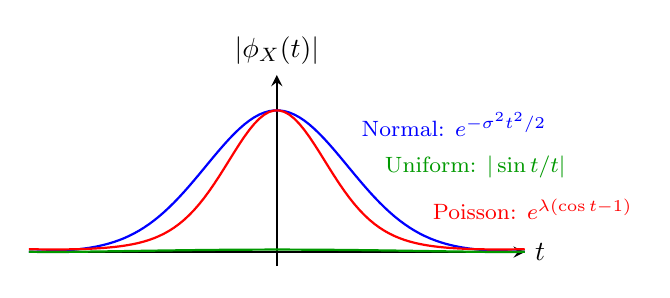
\begin{tikzpicture}[scale=0.9]

  \draw[->, thick, >=stealth] (-3.5,0) -- (3.5,0) node[right] {$t$};
  \draw[->, thick, >=stealth] (0,-0.2) -- (0,2.5) node[above] {$|\phi_X(t)|$};

  \draw[thick, blue, domain=-3.5:3.5, samples=100] plot (\x, {2*exp(-\x*\x/2)});
  \node[blue, font=\footnotesize] at (2.5,1.8) {Normal: $e^{-\sigma^2t^2/2}$};

  \draw[thick, red, domain=-3.5:3.5, samples=100] plot (\x, {2*exp(-2*(1-cos(\x r)))});
  \node[red, font=\footnotesize, xshift=1cm] at (2.5,0.6) {Poisson: $e^{\lambda(\cos t-1)}$};

  \draw[thick, green!60!black, domain=-3.5:3.5, samples=100] plot (\x, {abs(sin(\x r)/(\x r))*2});
  \node[green!60!black, font=\footnotesize] at (2.8,1.2) {Uniform: $|\sin t/t|$};
\end{tikzpicture}
\caption{The modulus $|\phi_X(t)|$ of the characteristic function for three distributions: normal (Gaussian decay), Poisson (periodic oscillatory decay) and uniform (sinc decay).}
\label{fig:characteristic_functions}
\end{figure}

\begin{lemma}[The positive-definiteness of the characteristic function]\label{ch14_characteristic_pd}
Let $\phi_X$ be the characteristic function of a random variable $X$. Then for any $n \in \mathbb{N}^+$, any $t_1, \dots, t_n \in \mathbb{R}$ and any complex numbers $z_1, \dots, z_n$,
\[
\sum_{j,k=1}^{n} z_j \overline{z_k}\, \phi_X(t_j - t_k) \ge 0,
\]
that is, the matrix $\bigl( \phi_X(t_j - t_k) \bigr)_{j,k=1}^{n}$ is positive semi-definite.
\end{lemma}

\begin{proof}
By Definition \ref{def:characteristic_function} and the linearity of the expectation:
\[
\sum_{j,k} z_j \overline{z_k}\, \phi_X(t_j - t_k)
= \mathbb{E}\Big[ \sum_{j,k} z_j \overline{z_k}\, e^{i(t_j - t_k) X} \Big]
= \mathbb{E}\Big[ \Big| \sum_{j} z_j e^{it_j X} \Big|^2 \Big] \ge 0.
\]
\end{proof}

\begin{example}[Explicit computation of the characteristic function of the Poisson distribution]\label{ch14_poisson_char_example}
Let $X \sim \operatorname{Poisson}(\lambda)$. Then
\[
\phi_X(t) = \sum_{k=0}^{\infty} e^{itk}\, \frac{\lambda^k e^{-\lambda}}{k!}
= e^{-\lambda} \sum_{k=0}^{\infty} \frac{(\lambda e^{it})^k}{k!}
= e^{\lambda (e^{it} - 1)}.
\]
Taking $\lambda = 2$ and $t = \pi/2$: $\phi_X(\pi/2) = e^{2(i-1)} = e^{-2} e^{2i} \approx 0.1353 \cdot (-0.4161 + 0.9093 i) \approx -0.0563 + 0.1230 i$. The modulus is $|\phi_X(\pi/2)| = e^{-2} \approx 0.1353$.
\end{example}

\begin{example}[Explicit computation of the characteristic function of the binomial distribution]\label{ch14_binomial_char_example}
Let $X \sim \operatorname{Binomial}(n, p)$. Then
\[
\phi_X(t) = (p e^{it} + 1 - p)^n.
\]
Taking $n = 3$ and $p = 1/2$: $\phi_X(t) = \tfrac18 (e^{it} + 1)^3$. Substituting $t = \pi$: $\phi_X(\pi) = (-\tfrac12 + \tfrac12)^3 = 0$, in agreement with direct summation.
\end{example}

\begin{example}[The characteristic function of the normal distribution]\label{ex:normal_characteristic}
If $X \sim \mathcal{N}(\mu, \sigma^2)$, then $\phi_X(t) = e^{i\mu t - \sigma^2 t^2/2}$. The modulus $|\phi_X(t)| = e^{-\sigma^2 t^2/2}$ is the Gaussian kernel. The argument $\arg \phi_X(t) = \mu t$ is a linear phase.
\end{example}

\begin{example}[The characteristic function of the gamma distribution]\label{ex:gamma_characteristic}
If $X \sim \operatorname{Gamma}(\alpha, \beta)$, then $\phi_X(t) = (1 - it/\beta)^{-\alpha}$ ($t \in \mathbb{R}$). The characteristic function of the exponential distribution ($\alpha = 1$) is $\phi_X(t) = (1 - it/\lambda)^{-1}$.
\end{example}

\begin{remark}[The values of the characteristic function at integer frequencies]\label{ch14_periodic_series_interface}
Let $X$ be a random variable on $S^1$ with mass density $f_X$. Then the Fourier coefficients of $f_X$ are
\[
c_n = \frac{1}{2\pi} \int_0^{2\pi} f_X(\theta)\, e^{-in\theta}\, d\theta = \frac{1}{2\pi}\mathbb{E}[e^{-inX}] = \frac{\phi_X(-n)}{2\pi}.
\]
That is, $c_n = \phi_X(-n)/(2\pi)$: the values of the characteristic function at integer frequencies are $2\pi$ times the Fourier coefficients of the density function. This correspondence is the core interface between periodic mathematics and probability theory: \textbf{the values of the characteristic function of a probability distribution at integer points are precisely $2\pi$ times the Fourier coefficients of its density}.
\end{remark}

\begin{proposition}[Characteristic function and Fourier coefficients of distributions on $S^1$]\label{prop:S1_char_fourier}
Let $X$ be a random variable on $S^1$ with density $f_X \in L^1(S^1)$. Then:
\begin{enumerate}[label=(\roman*)]
    \item the conjugate normalised characteristic function $\phi_X(-n)/(2\pi)$ consists of the Fourier coefficients $c_n$ of the density, that is, $\phi_X(-n) = 2\pi c_n$ (equivalently $\phi_X(n) = 2\pi c_{-n}$, $n \in \mathbb{Z}$);
    \item the density can be reconstructed from the characteristic function: $f_X(\theta) = \frac{1}{2\pi}\sum_{n \in \mathbb{Z}} \phi_X(n) e^{in\theta}$ (in the $L^2$ sense);
    \item Parseval's identity: $\sum_{n \in \mathbb{Z}} |\phi_X(n)|^2 = 2\pi \int_{S^1} |f_X(\theta)|^2 d\theta$.
\end{enumerate}
\end{proposition}

\begin{proof}
(i) Directly from Definition \ref{def:characteristic_function} and the definition of the Fourier coefficients. (ii) From the inverse Fourier transform formula. (iii) From Parseval's identity on $L^2(S^1)$.
\end{proof}

\section{Bayesian Inference}\label{sec:bayesian_inference}

\subsection{The Basic Framework of Bayesian Inference}
\label{subsec:bayes_framework}

\begin{definition}[The basic framework of Bayesian inference]\label{def:bayesian_inference}
\textbf{Bayesian inference} is the method of treating an unknown parameter $\theta$ as a random variable and updating one's knowledge of $\theta$ through observed data $\mathbf{D}$. Its three basic elements are:
\begin{enumerate}[label=(\roman*)]
    \item \textbf{Prior distribution} $\pi(\theta)$: the distribution before observation.
    \item \textbf{Likelihood function} $p(\mathbf{D} \mid \theta)$: the probability of the observed data given the parameter $\theta$.
    \item \textbf{Posterior distribution} $p(\theta \mid \mathbf{D})$: the distribution after observation, given by Bayes' theorem:
    \[
    p(\theta \mid \mathbf{D}) = \frac{p(\mathbf{D} \mid \theta) \pi(\theta)}{p(\mathbf{D})}.
    \]
\end{enumerate}
\end{definition}

\begin{definition}[Conjugate prior]\label{def:conjugate_prior}
Let $\mathcal{F} = \{p(\mathbf{D} \mid \theta)\}$ be a family of likelihood functions. A family of prior distributions $\mathcal{G}$ is called a \textbf{conjugate prior} family for $\mathcal{F}$ if, for every $\pi \in \mathcal{G}$ and every data set $\mathbf{D}$, the posterior $p(\theta \mid \mathbf{D})$ still belongs to $\mathcal{G}$. A conjugate prior is a family of distributions closed under Bayesian updating.
\end{definition}

\begin{figure}[htbp]
\centering
\begin{tikzpicture}[font=\small, arr/.style={->, thick, >=stealth}]
  \node[draw, rounded corners, fill=blue!8, minimum width=2.6cm, minimum height=0.8cm] (prior) {Prior $\pi(\theta)$};
  \node[draw, rounded corners, fill=orange!12, minimum width=2.6cm, minimum height=0.8cm, right=1.0cm of prior] (like) {Likelihood $p(\mathbf D|\theta)$};
  \node[draw, rounded corners, fill=green!12, minimum width=2.6cm, minimum height=0.8cm, right=1.0cm of like] (post) {Posterior $p(\theta|\mathbf D)$};
  \draw[arr] (prior) -- (like);
  \draw[arr] (like) -- (post);
  \node[font=\footnotesize] at (3,-1.0) {Bayesian updating: prior $\times$ likelihood $\propto$ posterior};
\end{tikzpicture}
\caption{The three elements of Bayesian inference: prior, likelihood and posterior.}
\label{fig:bayes_framework}
\end{figure}

\begin{example}[The Beta--binomial conjugate model]\label{ex:beta_binomial}
Let the likelihood be $X \mid \theta \sim \operatorname{Binomial}(n, \theta)$ and the prior be $\theta \sim \operatorname{Beta}(\alpha, \beta)$. Then the posterior is $\theta \mid X = x \sim \operatorname{Beta}(\alpha + x, \beta + n - x)$. The prior parameters $(\alpha, \beta)$ are updated to $(\alpha + x, \beta + n - x)$---the `pseudo-observation counts' of the prior are added to the actual observation counts.
\end{example}

\begin{example}[A numerical example of Beta--binomial conjugate updating]\label{ch14_beta_binomial_numeric}
Let the likelihood be $X \mid \theta \sim \operatorname{Binomial}(10, \theta)$ and the prior be $\theta \sim \operatorname{Beta}(2, 2)$, and suppose that $x = 7$ successes are observed. The posterior is $\theta \mid X = 7 \sim \operatorname{Beta}(9, 5)$.
\begin{itemize}
    \item prior mean: $\mathbb{E}[\theta] = 0.5$; posterior mean: $\mathbb{E}[\theta \mid \mathbf{D}] = 9/14 \approx 0.6429$;
    \item posterior variance: $\operatorname{Var}(\theta \mid \mathbf{D}) = 3/196 \approx 0.01531$;
    \item posterior mode: $2/3 \approx 0.6667$.
\end{itemize}
The prior pseudo-counts $(1, 1)$ and the actual observations $(7, 3)$ add to give the posterior pseudo-counts $(8, 6)$.
\end{example}

\begin{example}[The normal--normal conjugate model]\label{ex:normal_normal}
Let the likelihood be $X_1, \dots, X_n \mid \mu \sim \mathcal{N}(\mu, \sigma^2)$ (with $\sigma^2$ known) and the prior be $\mu \sim \mathcal{N}(\mu_0, \tau^2)$. Then the posterior is
\[
\mu \mid \mathbf{D} \sim \mathcal{N}\left( \frac{\frac{1}{\tau^2}\mu_0 + \frac{n}{\sigma^2}\bar{x}}{\frac{1}{\tau^2} + \frac{n}{\sigma^2}}, \; \frac{1}{\frac{1}{\tau^2} + \frac{n}{\sigma^2}} \right).
\]
\end{example}

\begin{example}[The gamma--Poisson conjugate model]
\label{ex:gamma_poisson}
Let the likelihood be
\[
X \mid \lambda \sim \operatorname{Poisson}(\lambda),
\]
and the prior be $\lambda \sim \operatorname{Gamma}(\alpha, \beta)$.
Then the posterior is
\[
\lambda \mid X = x \sim \operatorname{Gamma}(\alpha + x, \beta + 1).
\]
The shape parameter of the prior is increased by the number of observations, and the rate parameter is increased by $1$.
\end{example}

\begin{definition}[Marginal likelihood]\label{def:marginal_likelihood}
\textbf{The marginal likelihood} is $p(\mathbf{D}) = \int_{\Theta} p(\mathbf{D} \mid \theta) \pi(\theta) d\theta$. The marginal likelihood is the overall integral of the prior distribution against the likelihood weights.
\end{definition}

\subsection{Sequential Bayesian Updating and Posterior Convergence}

\begin{definition}[Sequential Bayesian updating]\label{def:sequential_bayesian}
Let the initial prior be $\pi_0(\theta)$ and let the observed data be $\mathbf{D}_1, \mathbf{D}_2, \dots$ in order. The sequential Bayesian update is
\[
p_k(\theta) \propto p(\mathbf{D}_k \mid \theta) p_{k-1}(\theta), \quad k = 1, 2, \dots.
\]
\end{definition}

\begin{theorem}[The Bernstein--von Mises theorem]\label{thm:bernstein_von_mises}
Let $\mathbf{D} = (X_1, \dots, X_n)$ be an independent and identically distributed sample, let $\theta_0$ be the true parameter, and let the prior $\pi(\theta)$ be continuous and positive at $\theta_0$. Then under suitable regularity conditions,
\[
\sqrt{n}(\theta - \hat{\theta}_n) \mid \mathbf{D} \xrightarrow{d} \mathcal{N}(0, \mathcal{I}(\theta_0)^{-1}).
\]
The posterior distribution converges to a normal distribution for large samples.
\end{theorem}

\begin{proof}[Sketch of proof]
The prior is approximately constant near $\theta_0$, and the posterior is proportional to the likelihood. Expanding the log-likelihood to second order at the maximum-likelihood estimate shows that the posterior density is asymptotically proportional to $\exp(-\tfrac12 \mathcal{I}(\theta_0) u^2)$, that is, to $\mathcal{N}(0, \mathcal{I}(\theta_0)^{-1})$. For a rigorous argument see van der Vaart, \emph{Asymptotic Statistics} (1998), Chapter 10.
\end{proof}

\begin{proposition}[Bayesian periodic-parameter estimation]\label{prop:bayesian_periodic_diagnosis}
For a stochastic process with periodic structure, Bayesian inference can be used to estimate the period parameters. The posterior $p(T \mid \mathbf{D})$ exhibits a sharp peak at the true period, and the maximum a posteriori estimate $\hat{T}_{\text{MAP}}$ gives the optimal estimate of the period. The width of the posterior measures the uncertainty of the estimate---the more samples there are, the narrower the posterior.
\end{proposition}

\begin{proof}
By the Bernstein--von Mises theorem (Theorem \ref{thm:bernstein_von_mises}),
the posterior is approximately
\[
\mathcal{N}\!\bigl(T_0, [n\mathcal{I}(T_0)]^{-1}\bigr),
\]
for large samples,
so the maximum a posteriori estimate converges in probability to $T_0$,
and the width of the posterior is $O(n^{-1/2})$.
\end{proof}

\section{Numerical Characteristics of Random Variables}\label{sec:numerical_characteristics}

\begin{definition}[Mathematical expectation]\label{def:mathematical_expectation}
The \textbf{mathematical expectation} of a random variable $X$ is
\[
\mathbb{E}[X] =
\begin{cases}
\sum_k k p_X(k) & \text{(discrete)} \\
\int_{-\infty}^{\infty} x f_X(x) dx & \text{(continuous)}
\end{cases}.
\]
\end{definition}

\begin{property}[Basic properties of the expectation]\label{prop:expectation_properties}
\begin{enumerate}[label=(\roman*)]
    \item \textbf{Linearity}: $\mathbb{E}[aX + bY] = a\mathbb{E}[X] + b\mathbb{E}[Y]$.
    \item \textbf{Multiplicativity under independence}: if $X, Y$ are independent, then $\mathbb{E}[XY] = \mathbb{E}[X]\mathbb{E}[Y]$.
    \item \textbf{Monotonicity}: if $X \le Y$ almost everywhere, then $\mathbb{E}[X] \le \mathbb{E}[Y]$.
\end{enumerate}
\end{property}

\begin{proof}
(i) By the linearity of the integral.

(ii) By independence, the joint distribution factorises,
\[
\mathbb{E}[XY]
= \int xy \, dF_X(x)\,dF_Y(y)
= \mathbb{E}[X]\,\mathbb{E}[Y].
\]

(iii) Since $Y - X \ge 0$ holds almost everywhere,
we obtain $\mathbb{E}[Y - X] \ge 0$.
\end{proof}

\begin{definition}[Variance and standard deviation]\label{def:variance_std}
\[
\operatorname{Var}(X) = \mathbb{E}[(X - \mathbb{E}[X])^2] = \mathbb{E}[X^2] - (\mathbb{E}[X])^2.
\]
The standard deviation is $\sigma_X = \sqrt{\operatorname{Var}(X)}$.
\end{definition}

\begin{property}[Basic properties of the variance]\label{prop:variance_properties}
\begin{enumerate}[label=(\roman*)]
    \item \textbf{Translation invariance}: $\operatorname{Var}(X + b) = \operatorname{Var}(X)$.
    \item \textbf{Covariance under scaling}: $\operatorname{Var}(aX) = a^2 \operatorname{Var}(X)$.
    \item \textbf{Additivity under independence}: if $X, Y$ are independent, then $\operatorname{Var}(X + Y) = \operatorname{Var}(X) + \operatorname{Var}(Y)$.
\end{enumerate}
\end{property}

\begin{proof}
(i) $\operatorname{Var}(X + b) = \mathbb{E}[(X + b - \mathbb{E}[X] - b)^2] = \operatorname{Var}(X)$. (ii) $\operatorname{Var}(aX) = \mathbb{E}[a^2(X - \mathbb{E}[X])^2] = a^2 \operatorname{Var}(X)$. (iii) By independence, $\operatorname{Var}(X + Y) = \mathbb{E}[(X - \mathbb{E}[X])^2] + \mathbb{E}[(Y - \mathbb{E}[Y])^2] + 2\mathbb{E}[(X - \mathbb{E}[X])(Y - \mathbb{E}[Y])] = \operatorname{Var}(X) + \operatorname{Var}(Y)$.
\end{proof}

\begin{definition}[Covariance and correlation coefficient]\label{def:covariance}
The \textbf{covariance} of random variables $X, Y$ is $\operatorname{Cov}(X, Y) = \mathbb{E}[(X - \mathbb{E}[X])(Y - \mathbb{E}[Y])]$. The \textbf{correlation coefficient} is $\rho_{XY} = \operatorname{Cov}(X, Y)/(\sigma_X \sigma_Y)$, taking values in $[-1, 1]$.
\end{definition}

\begin{definition}[Moments, skewness, and kurtosis]\label{def:moments}
The $k$-th raw moment is $\mu_k' = \mathbb{E}[X^k]$ and the $k$-th central moment is $\mu_k = \mathbb{E}[(X - \mu)^k]$. The \textbf{skewness} is $\gamma_1 = \mu_3/\sigma^3$ and the \textbf{kurtosis} is $\gamma_2 = \mu_4/\sigma^4 - 3$.
\end{definition}

\begin{definition}[Entropy]\label{def:entropy}
The \textbf{entropy} of a discrete random variable $X$ is $H(X) = -\sum_x p(x) \log p(x)$. The \textbf{differential entropy} of a continuous random variable $X$ is $h(X) = -\int f(x) \log f(x) dx$. Entropy measures the uniformity of a distribution.
\end{definition}

\begin{proposition}[The maximum entropy of the uniform distribution]\label{prop:uniform_max_entropy}
On $C_N$, the distribution with maximum entropy is the uniform distribution $p(k) = 1/N$, with maximum entropy $H_{\max} = \log N$.
\end{proposition}

\begin{proof}
By the logarithmic inequality $\log x \ge 1 - \frac{1}{x}$ ($x > 0$), taking $x = N p_k$:
\[
\sum_{k} p_k \log(N p_k) \ge \sum_{k} p_k \Bigl( 1 - \frac{1}{N p_k} \Bigr) = 1 - 1 = 0.
\]
Expanding gives $\log N - H(p) \ge 0$, that is, $H(p) \le \log N$. Equality holds if and only if $p_k = 1/N$ for all $k$.
\end{proof}

\section{The Laws of Large Numbers and the Central Limit Theorem}\label{sec:lln_clt}

\begin{theorem}[The weak law of large numbers]\label{thm:weak_law_of_large_numbers}
Let $X_1, X_2, \dots$ be independent and identically distributed random variables with $\mathbb{E}[X_i] = \mu$ and $\operatorname{Var}(X_i) = \sigma^2 < \infty$. Then for any $\varepsilon > 0$,
\[
\lim_{n \to \infty} \mathbb{P}(|\bar{X}_n - \mu| > \varepsilon) = 0.
\]
The sample mean converges in probability to the population mean.
\end{theorem}

\begin{proof}
By the independent and identically distributed property, $\mathbb{E}[\bar{X}_n] = \mu$ and $\operatorname{Var}(\bar{X}_n) = \sigma^2/n$. By Chebyshev's inequality,
\[
\mathbb{P}(|\bar{X}_n - \mu| > \varepsilon) \le \frac{\sigma^2}{n\varepsilon^2} \to 0.
\]
\end{proof}

\begin{theorem}[The central limit theorem]\label{thm:central_limit_theorem}
Let $X_1, X_2, \dots$ be independent and identically distributed random variables with $\mathbb{E}[X_i] = \mu$ and $\operatorname{Var}(X_i) = \sigma^2 < \infty$. Let $Z_n = \frac{\sum_{i=1}^n X_i - n\mu}{\sigma\sqrt{n}}$. Then $Z_n$ converges in distribution to the standard normal distribution.
\end{theorem}

\begin{proof}
Let $Y_i = (X_i - \mu)/\sigma$; then $\mathbb{E}[Y_i] = 0$ and $\operatorname{Var}(Y_i) = 1$. Expand the characteristic function $\phi_Y(s)$ in a Taylor series at $s = 0$: $\phi_Y(s) = 1 - s^2/2 + o(s^2)$. By independence,
\[
\phi_{Z_n}(t) = [\phi_Y(t/\sqrt{n})]^n = [1 - t^2/(2n) + o(1/n)]^n \to e^{-t^2/2}.
\]
$e^{-t^2/2}$ is the characteristic function of the standard normal distribution, and the result follows from Lévy's continuity theorem.
\end{proof}

\begin{figure}[htbp]
\centering
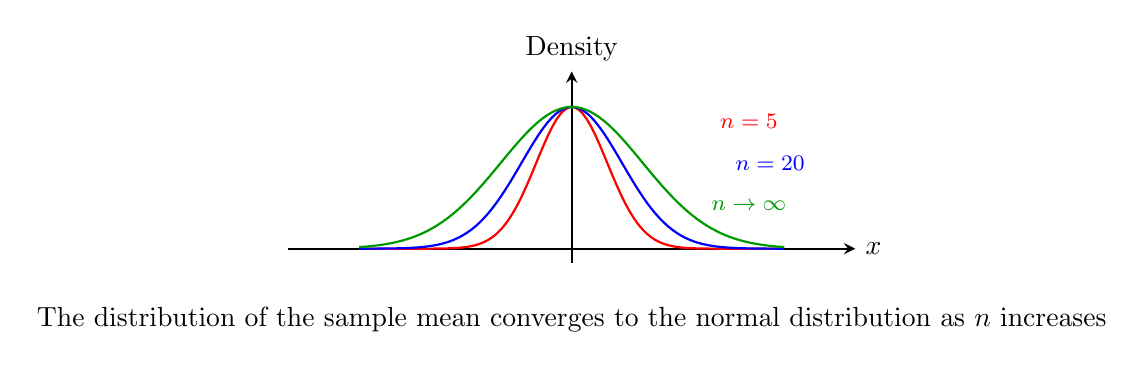
\begin{tikzpicture}[scale=0.9]
  % Coordinate axes
  \draw[->, thick, >=stealth] (-4,0) -- (4,0) node[right] {$x$};
  \draw[->, thick, >=stealth] (0,-0.2) -- (0,2.5) node[above] {Density};
  % Distribution of the sample mean (n increasing)
  \draw[thick, red, domain=-3:3, samples=100] plot (\x, {2*exp(-\x*\x/0.5)});
  \node[red, font=\footnotesize] at (2.5,1.8) {$n=5$};
  \draw[thick, blue, domain=-3:3, samples=100] plot (\x, {2*exp(-\x*\x/1)});
  \node[blue, font=\footnotesize] at (2.8,1.2) {$n=20$};
  \draw[thick, green!60!black, domain=-3:3, samples=100] plot (\x, {2*exp(-\x*\x/2)});
  \node[green!60!black, font=\footnotesize] at (2.5,0.6) {$n\to\infty$};
  % Annotation
  \node at (0,-1.0) {The distribution of the sample mean converges to the normal distribution as $n$ increases};
\end{tikzpicture}
\caption{Illustration of the central limit theorem: the distribution of the sample mean converges to the normal distribution as $n$ increases.}
\label{fig:clt}
\end{figure}

\section{Foundations of Stochastic Processes}\label{sec:stochastic_processes}

\begin{definition}[Stochastic process]\label{def:stochastic_process}
A \textbf{stochastic process} is a family of random variables $\{X_t\}_{t \in \mathcal{T}}$, where $\mathcal{T}$ is an index set (usually taken to be $\mathbb{Z}$, $\mathbb{N}$ or $\mathbb{R}$).
\end{definition}

\subsection{Stationary Processes}

\begin{definition}[Stationary process]\label{def:stationary_process}
A stochastic process $\{X_t\}$ is called \textbf{weakly stationary} if $\mu(t) \equiv \mu$ and $\gamma(s, t) = \gamma(s-t)$. Stationarity is the realisation of time-translation invariance in stochastic processes.
\end{definition}

\begin{definition}[Power spectral density]\label{def:power_spectral_density}
Let $\{X_t\}$ be a weakly stationary process with autocovariance function $\gamma(h)$. The \textbf{power spectral density} is
\[
S(\omega) = \sum_{h=-\infty}^{\infty} \gamma(h) e^{-i\omega h}.
\]
$S(\omega)$ is the Fourier transform of the autocovariance function. This definition adopts the \textbf{delayed} convention (with exponent $-i\omega h$), which belongs to the same notation as Theorem \ref{thm:spectrum_classical_limit} of the `Harmonic Analysis' chapter; for the conversion between the two conventions see Remark \ref{rem:autocorrelation_two_conventions}.
\end{definition}

\begin{proposition}[Invariance of the Second Derivative of the Autocovariance of a Stationary Process]\label{ch14_autocovariance_stationarity}
Let $\{X_t\}$ be a weakly stationary process whose autocovariance function $\gamma(h)$ is twice differentiable at $h = 0$. Define $P = -\gamma''(0)$. Then the time-translation invariance of the stationary process implies that $P$ is independent of time.
\end{proposition}

\begin{proof}
A time translation $\tau$ maps the process to $\{X_{t+\tau}\}$. Stationarity guarantees that $\gamma_{\tau}(h) = \gamma(h)$ is independent of $\tau$, hence $P_{\tau} = -\gamma_{\tau}''(0) = -\gamma''(0) = P$. Here `invariance' is the direct equivalent statement of stationarity $\gamma(s, t) = \gamma(s - t)$.
\end{proof}

\begin{proposition}[Non-negativity of the power spectrum and Herglotz's theorem]\label{prop:power_spectrum_positive}
The autocovariance function $\gamma(h)$ of a weakly stationary process is a positive-definite sequence, and its power spectral density satisfies $S(\omega) \ge 0$. Conversely, any non-negative function $S$ satisfying $\int S(\omega) d\omega < \infty$ is the power spectrum of some weakly stationary process. This is the content of Herglotz's theorem.
\end{proposition}

\begin{proof}
Positive definiteness follows by the method of Proposition \ref{prop:characteristic_function_properties}: $\sum_{j,k} z_j \bar z_k \gamma(j-k) = \mathbb{E}|\sum_j z_j X_j|^2 \ge 0$. That $S(\omega) \ge 0$ follows from the fact that $S$ is the Fourier transform of a positive-definite sequence. The converse conclusion is given by the spectral measure theorem.
\end{proof}

\begin{figure}[htbp]
\centering
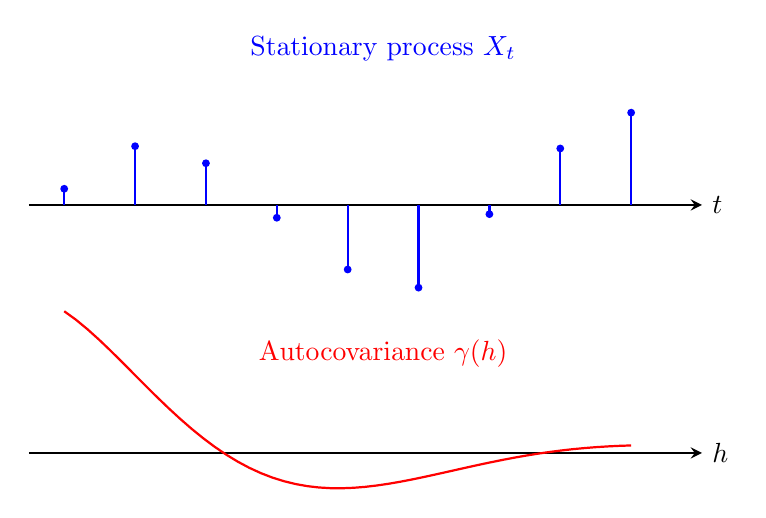
\begin{tikzpicture}[scale=0.9]
  % Time series
  \draw[->, thick, >=stealth] (-0.5,0) -- (9,0) node[right] {$t$};
  \foreach \x in {0,1,2,3,4,5,6,7,8} {
    \pgfmathsetmacro{\y}{1.2*sin(\x*60)+0.5*rand}
    \draw[thick, blue] (\x,0) -- (\x,\y);
    \node[circle, fill, blue, inner sep=1pt] at (\x,\y) {};
  }
  \node[blue] at (4.5,2.2) {Stationary process $X_t$};
  % Autocovariance
  \begin{scope}[shift={(0,-3.5)}]
    \draw[->, thick, >=stealth] (-0.5,0) -- (9,0) node[right] {$h$};
    \draw[thick, red, domain=0:8, samples=50] plot (\x, {2*exp(-\x/3)*cos(\x*40)});
    \node[red] at (4.5,1.4) {Autocovariance $\gamma(h)$};
  \end{scope}
\end{tikzpicture}
\caption{A stationary process and its autocovariance function: the autocovariance depends only on the time lag $h$.}
\label{fig:stationary_process}
\end{figure}

\subsection{Cyclostationary Processes}

\begin{definition}[Cyclostationary Process]\label{ch14_cyclostationary}
A stochastic process $\{X_t\}$ is called a \textbf{cyclostationary process} with period $T$ if its statistical properties are invariant under the time translation $t \mapsto t + T$. A stationary process is a special case of a cyclostationary process: it satisfies period-translation invariance for every $T$. Cyclostationarity belongs to the invariance of time-translation symmetry ($0$-symmetry) under the action of the periodic subgroup $T\mathbb{Z}$.
\end{definition}

\begin{proposition}[Fourier decomposition of cyclostationary processes]\label{prop:cyclostationary_fourier}
Let $\{X_t\}$ be a cyclostationary process with period $T$. Then its autocovariance function $\gamma(t, s) = \gamma(t+T, s+T)$ can be expanded as a double Fourier series:
\[
\gamma(t, s) = \sum_{n, m \in \mathbb{Z}} \gamma_{n,m} e^{i 2\pi n t/T} e^{-i 2\pi m s/T}.
\]
Here the $\gamma_{n,m}$ are the cyclic spectral coefficients. When $n = m$, the coefficients $\gamma_{n,n}$ constitute the stationary power spectrum.
\end{proposition}

\begin{proof}
By cyclostationarity, $\gamma(t, s)$ is periodic with respect to $(t, s)$ with period $T$. Expansion in Fourier series gives the double series. The stationary case ($T \to 0$) degenerates to $\gamma(t-s)$.
\end{proof}

\begin{figure}[htbp]
\centering
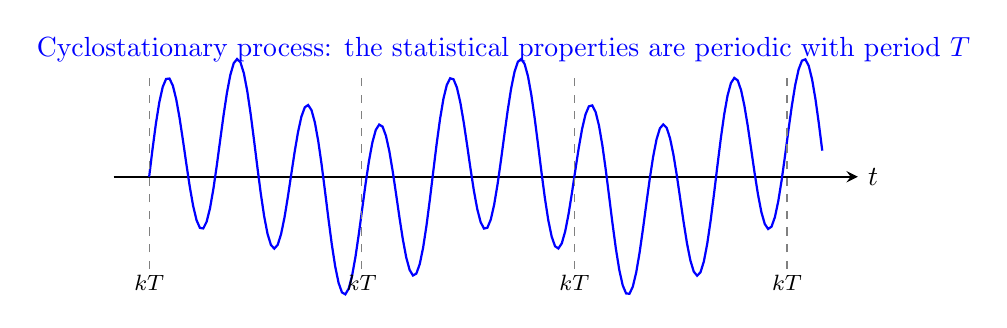
\begin{tikzpicture}[scale=0.9]
  % Cyclostationary signal
  \draw[->, thick, >=stealth] (-0.5,0) -- (10,0) node[right] {$t$};
  \draw[thick, blue, domain=0:9.5, samples=200] plot (\x, {1.2*sin(\x*360)+0.5*sin(\x*90)});
  \node[blue] at (5,1.8) {Cyclostationary process: the statistical properties are periodic with period $T$};
  % Period markers
  \foreach \x in {0,3,6,9} {
    \draw[gray, dashed] (\x,-1.3) -- (\x,1.5);
    \node[font=\footnotesize] at (\x,-1.5) {$kT$};
  }
\end{tikzpicture}
\caption{Cyclostationary process: the statistical properties are invariant under the period translation $t\mapsto t+T$.}
\label{fig:cyclostationary}
\end{figure}

\subsection{Markov Processes}

\begin{definition}[Markov Process]\label{def:markov_process}
A stochastic process $\{X_t\}$ is called a \textbf{Markov process} if
\[
\mathbb{P}(X_{t_n} \le x \mid X_{t_1}, \dots, X_{t_{n-1}}) = \mathbb{P}(X_{t_n} \le x \mid X_{t_{n-1}}).
\]
\end{definition}

\begin{lemma}[Spectral Radius Bound for Eigenvalues of a Stochastic Matrix]\label{ch14_transition_spectral_radius}
Let $P$ be a stochastic matrix on $C_N$. Then every eigenvalue $\lambda$ of $P$ satisfies $|\lambda| \le 1$, and $\lambda_0 = 1$ is an eigenvalue of $P$.
\end{lemma}

\begin{proof}
$\lambda_0 = 1$: $(P\mathbf{1})_i = \sum_j P_{ij} = 1$. $|\lambda| \le 1$: let $P\mathbf{v} = \lambda\mathbf{v}$ and take $|v_m| = \max_j |v_j| > 0$; then $|\lambda||v_m| \le \sum_j P_{mj}|v_j| \le |v_m|$, so $|\lambda| \le 1$.
\end{proof}

\begin{proposition}[Transition Operator and Eigenvalue Decomposition]\label{prop:transfer_operator_eigen}
Let $P$ be a Markov transition matrix on $C_N$ with eigenvalues $\lambda_0 = 1 \ge |\lambda_1| \ge \dots \ge |\lambda_{N-1}|$.
\begin{enumerate}[label=(\roman*)]
    \item $\lambda_0 = 1$: the invariant distribution---the fixed point of the distribution.
    \item $|\lambda_i| < 1$: decaying modes---the rate of convergence to the stationary distribution.
    \item $|\lambda_i| = 1$ with $\lambda_i \neq 1$: periodic modes---the distribution cycles among several states.
\end{enumerate}
\end{proposition}

\begin{proof}
(i) A distribution $\pi$ satisfying $\pi P = \pi$, $\pi \ge 0$ and $\sum_i \pi_i = 1$ is an invariant distribution. (ii) When $|\lambda_i| < 1$ the corresponding mode decays as $|\lambda_i|^n \to 0$. (iii) If $\lambda_i$ is a $k$-th root of unity, then the mode cycles among $k$ states, corresponding to a periodic pattern of period $k$.
\end{proof}

\begin{proposition}[Period of irreducible Markov chains]\label{prop:markov_chain_period}
Let $P$ be the transition matrix of a finite Markov chain. If the chain is irreducible and aperiodic (that is, all eigenvalues other than $\lambda_0=1$ satisfy $|\lambda_i|<1$), then the chain converges to the stationary distribution at an exponential rate:
\[
\|P^n \pi_0 - \pi\| \le C \rho^n, \quad \rho = \max_{i \ge 1} |\lambda_i| < 1.
\]
If the chain has period $d > 1$, then the eigenvalues $e^{2\pi i k/d}$ ($k=0,\dots,d-1$) all have modulus $1$, and the chain cycles among $d$ classes of states.
\end{proposition}

\begin{proof}
By the Perron--Frobenius theorem, for an irreducible aperiodic chain the spectral radius $1$ is a simple eigenvalue, and the remaining eigenvalues have modulus strictly less than $1$. The rate of convergence is determined by the modulus $|\lambda_1|$ of the second largest eigenvalue. The periodic case follows by decomposing $P^d$ into $d$ aperiodic subchains.
\end{proof}

\begin{example}[Eigenvalues and Period of a Three-State Permutation Chain]\label{ch14_markov_cycle_example}
Consider the permutation transition matrix on $C_3$
\[
P = \begin{pmatrix} 0 & 1 & 0 \\ 0 & 0 & 1 \\ 1 & 0 & 0 \end{pmatrix}.
\]
Its characteristic polynomial is $\lambda^3 - 1$, with eigenvalues $\lambda_0 = 1$, $\lambda_1 = e^{2\pi i/3}$ and $\lambda_2 = e^{4\pi i/3}$. The moduli of the three eigenvalues are all $1$, corresponding to a cyclic mode of period $3$. The invariant distribution is $\pi = (1/3, 1/3, 1/3)$.
\end{example}

\begin{figure}[htbp]
\centering
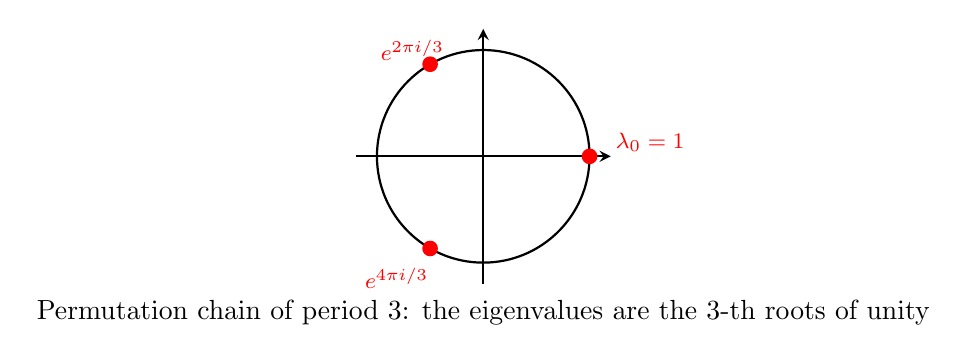
\begin{tikzpicture}[scale=0.9]

  \draw[thick] (0,0) circle (1.5);
  \draw[->, thick, >=stealth] (-1.8,0) -- (1.8,0);
  \draw[->, thick, >=stealth] (0,-1.8) -- (0,1.8);

  \node[circle, fill, red, inner sep=2pt] at (1.5,0) {};
  \node[circle, fill, red, inner sep=2pt] at (-0.75,1.30) {};
  \node[circle, fill, red, inner sep=2pt] at (-0.75,-1.30) {};
  \node[red, font=\footnotesize, xshift=0.5cm] at (1.8,0.2) {$\lambda_0=1$};
  \node[red, font=\footnotesize] at (-1.0,1.5) {$e^{2\pi i/3}$};
  \node[red, font=\footnotesize, xshift=-0.2cm, yshift=-0.2cm] at (-1.0,-1.5) {$e^{4\pi i/3}$};
  \node at (0,-2.2) {Permutation chain of period $3$: the eigenvalues are the $3$-th roots of unity};
\end{tikzpicture}
\caption{The eigenvalues of the permutation chain of period $3$ are distributed on the unit circle, corresponding to the periodic cyclic mode of the distribution.}
\label{fig:markov_cycle}
\end{figure}

\subsection{Brownian Motion}

\begin{definition}[Brownian Motion]\label{def:brownian_motion}
\textbf{Standard Brownian motion} $\{W_t\}_{t \ge 0}$ satisfies: $W_0 = 0$, the increments are independent, $W_t - W_s \sim \mathcal{N}(0, t-s)$, and the sample paths are continuous. Brownian motion is self-similar: $\{W_{\lambda t}\} \stackrel{d}{=} \{\sqrt{\lambda} W_t\}$.
\end{definition}

\begin{definition}[Self-Similarity and the Scaling Exponent]\label{ch14_scale_invariance}
A stochastic process $\{X_t\}$ is called \textbf{self-similar} if there exists $H > 0$ such that $\{X_{\lambda t}\} \stackrel{d}{=} \{\lambda^H X_t\}$ for all $\lambda > 0$. The number $H$ is called the \textbf{Hurst exponent} (or self-similarity exponent). For Brownian motion $H = 1/2$.

The \textbf{tail exponent} $\alpha > 0$ of a heavy-tailed distribution is defined by $\mathbb{P}(|X| > x) \sim x^{-\alpha}$. The Hurst exponent and the tail exponent are characteristic invariants of a distribution or a process under scaling transformations.
\end{definition}

\begin{figure}[htbp]
\centering
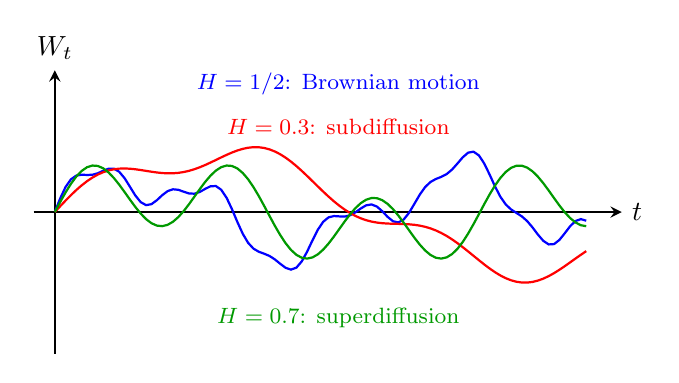
\begin{tikzpicture}[scale=0.9]
  % Brownian motion path
  \draw[->, thick, >=stealth] (-0.3,0) -- (8,0) node[right] {$t$};
  \draw[->, thick, >=stealth] (0,-2) -- (0,2) node[above] {$W_t$};
  % Three self-similar paths
  \draw[thick, blue, domain=0:7.5, samples=100] plot (\x, {0.5*sin(\x*80)+0.3*sin(\x*200)+0.1*sin(\x*500)});
  \node[blue, font=\footnotesize] at (4,1.8) {$H=1/2$: Brownian motion};
  \draw[thick, red, domain=0:7.5, samples=100] plot (\x, {0.8*sin(\x*40)+0.2*sin(\x*150)});
  \node[red, font=\footnotesize] at (4,1.2) {$H=0.3$: subdiffusion};
  \draw[thick, green!60!black, domain=0:7.5, samples=100] plot (\x, {0.3*sin(\x*60)+0.5*sin(\x*180)});
  \node[green!60!black, font=\footnotesize] at (4,-1.5) {$H=0.7$: superdiffusion};
\end{tikzpicture}
\caption{The Hurst exponent of a self-similar process and the roughness of its sample paths: the smaller $H$ is, the rougher the path.}
\label{fig:self_similar}
\end{figure}

\section{Transformation Groups and Ergodicity in Probability Spaces}\label{sec:ergodicity}

\begin{definition}[Measure-Preserving Transformation]\label{def:measure_preserving}
A mapping $T: \Omega \to \Omega$ is called a \textbf{measure-preserving transformation} if $\mathbb{P}(T^{-1}(A)) = \mathbb{P}(A)$ for every $A \in \mathcal{F}$.
\end{definition}

\begin{definition}[Ergodicity]\label{def:ergodicity}
A measure-preserving transformation $T$ is called \textbf{ergodic} if every $T$-invariant event $A$ satisfies $\mathbb{P}(A) \in \{0, 1\}$.
\end{definition}

\begin{theorem}[Birkhoff Ergodic Theorem]\label{thm:birkhoff_ergodic}
Let $T$ be a measure-preserving transformation and $f \in L^1(\mathbb{P})$. Then the time average
\[
\bar{f}(\omega) = \lim_{n \to \infty} \frac{1}{n} \sum_{k=0}^{n-1} f(T^k \omega)
\]
exists almost everywhere, and $\mathbb{E}[\bar{f}] = \mathbb{E}[f]$. If $T$ is ergodic, then $\bar{f}(\omega) = \mathbb{E}[f]$ holds almost everywhere.
\end{theorem}

\begin{proof}[Sketch of proof]
The standard argument: first prove the maximal ergodic inequality, then prove the almost-everywhere convergence of the time averages, and finally use ergodicity to identify the limit as the space average. For details see Walters, \emph{An Introduction to Ergodic Theory} (1982), Chapter 1.
\end{proof}

\begin{corollary}[Time-Average--Space-Average Criterion of the Ergodic Theorem]\label{cor:ergodic_closure}
For an ergodic measure-preserving transformation the time average equals the space average, which means that the long-term behaviour of a single orbit fully characterises the whole probability space. Ergodicity is the mathematical formulation of `the orbit being dense in the sample space'.
\end{corollary}

\begin{proof}
By Theorem \ref{thm:birkhoff_ergodic}, in the ergodic case $\bar{f}(\omega) = \mathbb{E}[f]$ holds almost everywhere, that is, the time average along every orbit converges to the space average.
\end{proof}

\begin{remark}[Scope and Limitations of the Ergodic Theorem]\label{ch14_ergodic_scope_remark}
The three conditions of Theorem \ref{thm:birkhoff_ergodic} each have their own limits: (i) measure preservation only guarantees that the time average exists, not that it equals the space average; (ii) ergodicity guarantees that a single orbit is a sufficient statistic for the whole sample space; (iii) integrability $f \in L^1(\mathbb{P})$ guarantees that $\bar{f}$ is integrable. When performing period diagnostics on a cyclostationary process, the ergodicity criterion should be applied to the phase-aligned process rather than to the original process.
\end{remark}

\begin{proposition}[Invariance under Three Time Scales]\label{prop:three_symmetry_stochastic}
\begin{enumerate}[label=(\roman*)]
    \item \textbf{Stationary processes (translation invariant, $0$-symmetry)}: the statistical properties are invariant under time translation.
    \item \textbf{Cyclostationary processes (period-translation invariant, the periodisation of $0$-symmetry)}: the statistical properties are invariant under the time translation $t \mapsto t + T$.
    \item \textbf{Self-similar processes (scale invariant, $1$-symmetry)}: the statistical properties are invariant under the scaling transformation $t \mapsto \lambda t$.
\end{enumerate}
\end{proposition}

\begin{proof}
(i) The statistical properties of a stationary process are invariant under time translation (Definition \ref{def:stationary_process}), and time translation is the action of the translation group $\mathbb{R}$ or $\mathbb{Z}$. (ii) The statistical properties of a cyclostationary process are invariant under the action of $T\mathbb{Z}$ (Definition \ref{ch14_cyclostationary}); the set $T\mathbb{Z}$ is a translation subgroup, so this is still translation symmetry. (iii) The statistical properties of a self-similar process are invariant under scaling transformations (Definition \ref{ch14_scale_invariance}), and a scaling transformation is the action of the scaling group $\mathbb{R}^+$. The three correspond respectively to invariance under a translation group, a translation subgroup and a scaling group.
\end{proof}

\section*{Seven-theme comparison table for this chapter}

\begin{figure}[htbp]
\centering
\begin{tikzpicture}[
  theme/.style={draw, rounded corners, fill=green!10, minimum width=1.2cm, minimum height=0.55cm, align=center, font=\footnotesize}
]
  \node[theme] (p) at (0,0) {Translation};
  \node[theme, right=0.3cm of p] (s) {Scaling};
  \node[theme, right=0.3cm of s] (r) {Rotation};
  \node[theme, right=0.3cm of r] (c) {Conservation};
  \node[theme, right=0.3cm of c] (sym) {Symmetry};
  \node[theme, right=0.3cm of sym] (cl) {Closure};
  \node[theme, right=0.3cm of cl] (per) {Period};
  \node[draw, dashed, rounded corners, fit=(p)(per), inner sep=6pt] (box) {};
  \node[below=0.1cm of box, font=\footnotesize] {The seven themes run through probability theory and distribution};
\end{tikzpicture}
\caption{The seven themes of this chapter: translation, scaling, rotation, conservation, symmetry, closure and period.}
\label{fig:probability_themes}
\end{figure}

\begin{center}
\renewcommand{\arraystretch}{1.3}
\begin{tabular}{>{\centering\arraybackslash}p{2.2cm}>{\centering\arraybackslash}p{10.5cm}}
\toprule
Theme & Corresponding content in this chapter \\
\midrule
Translation & The time-translation invariance of stationary processes (Definition \ref{def:stationary_process}); the period-translation invariance of cyclostationary processes (Definition \ref{ch14_cyclostationary}); the advance of sequential Bayesian updating along the time axis (Definition \ref{def:sequential_bayesian}) \\
Scaling & The scale invariance of self-similar processes and heavy-tailed distributions (Definition \ref{ch14_scale_invariance}); the scaling convergence of the central limit theorem (Theorem \ref{thm:central_limit_theorem}) \\
Rotation & The phase information of the argument of the characteristic function (Remark \ref{prop:characteristic_grammar}); the rotational symmetry of the uniform distribution on $S^1$ (Definition \ref{def:uniform_distribution}, Proposition \ref{prop:S1_uniform_rotation}) \\
Conservation & The invariance of the autocovariance under time translation (Proposition \ref{ch14_autocovariance_stationarity}); the invariance of the scaling exponent under scaling transformations \\
Symmetry & The closure of the family of conjugate priors (Definition \ref{def:conjugate_prior}); the prior/likelihood/posterior tripartite structure \\
Closure & The convergence closure of the laws of large numbers and the central limit theorem (Theorem \ref{thm:weak_law_of_large_numbers}, \ref{thm:central_limit_theorem}); the `time average = space average' criterion for ergodic orbits (Theorem \ref{thm:birkhoff_ergodic}) \\
Period & The period $T$ of a cyclostationary process (Definition \ref{ch14_cyclostationary}); the periodic pattern of Markov-chain eigenvalues with $|\lambda_i|=1$ (Proposition \ref{prop:transfer_operator_eigen}); the characteristic function and Fourier coefficients of distributions on $S^1$ (Proposition \ref{prop:S1_char_fourier}) \\
\bottomrule
\end{tabular}
\end{center}

\section*{Exercises}

\begin{enumerate}[leftmargin=3em, label=\textbf{Exercise \arabic*}]
    \item Prove the basic properties of the probability measure (Proposition \ref{prop:probability_measure_properties}):
    \begin{enumerate}[label=(\roman*)]
        \item $\mathbb{P}(\emptyset)=0$;
        \item monotonicity: $A\subseteq B\Rightarrow\mathbb{P}(A)\le\mathbb{P}(B)$;
        \item complementarity: $\mathbb{P}(A^c)=1-\mathbb{P}(A)$;
        \item finite additivity: $A\cap B=\emptyset\Rightarrow\mathbb{P}(A\cup B)=\mathbb{P}(A)+\mathbb{P}(B)$.
    \end{enumerate}
    Carry out the proof using the axiom of countable additivity, and explain why these four properties are necessary consequences of a probability measure.

    \item According to Definition \ref{def:frequency_probability}, explain the relation between frequency and probability:
    the frequency $f_n(A)=n_A/n$ of $A$ converges in probability to $\mathbb{P}(A)$.
    Explain the meaning of this convergence in the light of the law of large numbers (Theorem \ref{thm:weak_law_of_large_numbers}),
    and explain that the frequency is the empirical estimate of the probability and the probability is the limit of the frequency.

    \item Prove the four basic properties of the cumulative distribution function (Proposition \ref{prop:cdf_properties}):
    monotone non-decrease, right continuity, limiting behaviour and interval probability.
    Write out the proofs separately, and explain the basis of the statement in Theorem \ref{thm:cdf_uniqueness}
    that `two random variables are identically distributed if and only if their cumulative distribution functions are equal'.

    \item Using Definition \ref{def:bernoulli_binomial} and Definition \ref{def:poisson_distribution},
    prove the limiting relation from the binomial distribution to the Poisson distribution:
    \[
    \operatorname{Binomial}(n,\lambda/n)\xrightarrow{d}\operatorname{Poisson}(\lambda)
    \quad(n\to\infty).
    \]
    Carry out the proof using the limit of the probability mass function or of the characteristic function.

    \item Verify the limits and special-case relations among common distributions in Proposition \ref{prop:distribution_relations}:
    \begin{enumerate}[label=(\roman*)]
        \item binomial to Poisson;
        \item binomial to normal (the De Moivre--Laplace theorem);
        \item gamma to normal;
        \item $t$ distribution to normal;
        \item beta to normal.
    \end{enumerate}
    State separately the parametric limit condition for each relation.

    \item Prove the basic properties of the characteristic function (Proposition \ref{prop:characteristic_function_properties}):
    \begin{enumerate}[label=(\roman*)]
        \item $\phi_X(0)=1$ and $|\phi_X(t)|\le1$;
        \item if $X$ and $Y$ are independent, then $\phi_{X+Y}(t)=\phi_X(t)\phi_Y(t)$;
        \item $\mathbb{E}[X^n]=i^{-n}\phi_X^{(n)}(0)$;
        \item the characteristic function determines the distribution uniquely;
        \item $\phi_{aX+b}(t)=e^{ibt}\phi_X(at)$.
    \end{enumerate}

    \item Verify Example \ref{ex:normal_characteristic} and Example \ref{ex:gamma_characteristic}:
    \begin{enumerate}[label=(\roman*)]
        \item if $X\sim\mathcal{N}(\mu,\sigma^2)$, then $\phi_X(t)=e^{i\mu t-\sigma^2t^2/2}$;
        \item if $X\sim\operatorname{Gamma}(\alpha,\beta)$, then $\phi_X(t)=(1-it/\beta)^{-\alpha}$.
    \end{enumerate}
    Write out the derivations, and explain that the modulus of the characteristic function of the normal distribution is a Gaussian kernel and its argument is a linear phase.

    \item Prove Proposition \ref{prop:S1_char_fourier}:
    let $X$ be a random variable on $S^1$ with density $f_X\in L^1(S^1)$; then
    \begin{enumerate}[label=(\roman*)]
        \item the conjugate normalised characteristic function $\phi_X(-n)/(2\pi)$ consists of the Fourier coefficients $c_n$ of the density, that is, $\phi_X(-n)=2\pi c_n$ (equivalently $\phi_X(n)=2\pi c_{-n}$);
        \item the density can be reconstructed from the characteristic function;
        \item Parseval's identity holds.
    \end{enumerate}
    Explain how this correspondence embodies the unification of probability distributions and Fourier analysis on the circle group.

    \item Prove the basic properties of the expectation and of the variance (Proposition \ref{prop:expectation_properties}
    and Proposition \ref{prop:variance_properties}):
    \begin{enumerate}[label=(\roman*)]
        \item linearity of the expectation: $\mathbb{E}[aX+bY]=a\mathbb{E}[X]+b\mathbb{E}[Y]$;
        \item multiplicativity under independence: $X,Y$ independent $\Rightarrow\mathbb{E}[XY]=\mathbb{E}[X]\mathbb{E}[Y]$;
        \item translation invariance of the variance: $\operatorname{Var}(X+b)=\operatorname{Var}(X)$;
        \item covariance of the variance under scaling: $\operatorname{Var}(aX)=a^2\operatorname{Var}(X)$;
        \item additivity of the variance: $X,Y$ independent $\Rightarrow\operatorname{Var}(X+Y)=\operatorname{Var}(X)+\operatorname{Var}(Y)$.
    \end{enumerate}

    \item Prove the maximum-entropy property of the uniform distribution (Proposition \ref{prop:uniform_max_entropy}):
    on $C_N$, the distribution with maximum entropy is the uniform distribution, with maximum entropy $H_{\max}=\log N$.
    Carry out the proof using the logarithmic inequality $\log x\ge1-1/x$,
    and explain how this result is related to `the uniform distribution is the Haar measure on the cyclic group'.

    \item Prove the central limit theorem (Theorem \ref{thm:central_limit_theorem}):
    let $X_1,X_2,\dots$ be independent and identically distributed,
    with $\mathbb{E}[X_i]=\mu$ and $\operatorname{Var}(X_i)=\sigma^2<\infty$;
    then
    \[
    Z_n=\frac{\sum_{i=1}^nX_i-n\mu}{\sigma\sqrt{n}}
    \xrightarrow{d}\mathcal{N}(0,1).
    \]
    Carry out the proof using the Taylor expansion of the characteristic function at $s=0$,
    $\phi_Y(s)=1-s^2/2+o(s^2)$.

    \item Verify Example \ref{ex:beta_binomial} and Example \ref{ex:normal_normal}:
    \begin{enumerate}[label=(\roman*)]
        \item the posterior update of the Beta--binomial conjugate model;
        \item the posterior update of the normal--normal conjugate model.
    \end{enumerate}
    Write out the expressions for the prior, the likelihood and the posterior in each case,
    and explain how a conjugate prior guarantees that the family of posterior distributions is closed under Bayesian updating.

    \item Prove the Bernstein--von Mises theorem (Theorem \ref{thm:bernstein_von_mises}):
    under suitable regularity conditions,
    \[
    \sqrt{n}(\theta-\hat{\theta}_n)\mid\mathbf{D}
    \xrightarrow{d}\mathcal{N}(0,\mathcal{I}(\theta_0)^{-1}).
    \]
    Explain the intuitive meaning of the convergence of the posterior distribution to a normal distribution for large samples,
    and indicate the significance of this conclusion for the Bayesian estimation of period parameters
    (see Proposition \ref{prop:bayesian_periodic_diagnosis}).

    \item Prove the non-negativity of the power spectrum of a stationary process and Herglotz's theorem (Proposition \ref{prop:power_spectrum_positive}):
    the autocovariance function $\gamma(h)$ of a weakly stationary process is a positive-definite sequence,
    and its power spectral density satisfies $S(\omega)\ge0$;
    conversely, any non-negative function $S$ satisfying $\int S(\omega)d\omega<\infty$
    is the power spectrum of some weakly stationary process.
    Carry out the proof of positive definiteness using $\mathbb{E}|\sum_jz_jX_j|^2\ge0$.

    \item Prove the Fourier decomposition of cyclostationary processes (Proposition \ref{prop:cyclostationary_fourier}):
    let $\{X_t\}$ be a cyclostationary process with period $T$; then its autocovariance function
    \[
    \gamma(t,s)=\sum_{n,m\in\mathbb{Z}}\gamma_{n,m}e^{i2\pi nt/T}e^{-i2\pi ms/T}.
    \]
    Explain that when $n=m$ the coefficients $\gamma_{n,n}$ constitute the stationary power spectrum,
    and explain how cyclostationarity corresponds to the invariance of time-translation symmetry under the periodic subgroup $T\mathbb{Z}$.

    \item Prove the transition operator and eigenvalue decomposition of a Markov chain (Proposition \ref{prop:transfer_operator_eigen}):
    let $P$ be a Markov transition matrix on $C_N$ with eigenvalues
    $\lambda_0=1\ge|\lambda_1|\ge\dots\ge|\lambda_{N-1}|$.
    Explain that:
    \begin{enumerate}[label=(\roman*)]
        \item $\lambda_0=1$ corresponds to the invariant distribution---the fixed point of the distribution;
        \item $|\lambda_i|<1$ corresponds to decaying modes that converge to the stationary distribution;
        \item $|\lambda_i|=1$ with $\lambda_i\neq1$ corresponds to periodic modes.
    \end{enumerate}

    \item Verify the eigenvalues and the period of the three-state permutation chain in Example \ref{ch14_markov_cycle_example}:
    \[
    P=\begin{pmatrix}0&1&0\\0&0&1\\1&0&0\end{pmatrix},
    \]
    the characteristic polynomial is $\lambda^3-1$, with eigenvalues $\lambda_0=1$,
    $\lambda_1=e^{2\pi i/3}$ and $\lambda_2=e^{4\pi i/3}$.
    Explain that the moduli of the three eigenvalues are all $1$, corresponding to a cyclic mode of period $3$.

    \item Prove the Birkhoff ergodic theorem (Theorem \ref{thm:birkhoff_ergodic}):
    let $T$ be a measure-preserving transformation and $f\in L^1(\mathbb{P})$; then the time average
    \[
    \bar{f}(\omega)=\lim_{n\to\infty}\frac{1}{n}\sum_{k=0}^{n-1}f(T^k\omega)
    \]
    exists almost everywhere, and $\mathbb{E}[\bar{f}]=\mathbb{E}[f]$;
    if $T$ is ergodic, then $\bar{f}(\omega)=\mathbb{E}[f]$ holds almost everywhere.
    Explain the closure meaning of `the time average equals the space average' in Corollary \ref{cor:ergodic_closure}.

    \item Synthesis problem: combining the characteristic function (Definition \ref{def:characteristic_function}),
    stationary processes (Definition \ref{def:stationary_process}),
    cyclostationary processes (Definition \ref{ch14_cyclostationary})
    and the ergodic theorem (Theorem \ref{thm:birkhoff_ergodic}),
    explain the confluence of probability theory and periodic mathematics on the following four levels:
    \begin{enumerate}[label=(\roman*)]
        \item the characteristic function of a probability distribution is precisely the Fourier transform of the distribution;
        \item the uniform distribution on $S^1$ is the Haar measure on the circle group;
        \item the time-translation invariance of stationary processes and the period-translation invariance of cyclostationary processes;
        \item the closure criterion `time average equals space average' for ergodic orbits.
    \end{enumerate}
    Indicate separately where these confluences are situated in the framework of periodic mathematics.
\end{enumerate}

